% UECM3034 Numerical Methods - combined course notes.
% Included by both UECM3034_Complete.tex and UECM3034_Student.tex.

\documentclass[12pt,a4paper]{report}

\usepackage[a4paper,top=2.5cm,bottom=2.4cm,left=2.55cm,right=2.55cm]{geometry}
\usepackage[T1]{fontenc}
\usepackage[utf8]{inputenc}
\usepackage{lmodern}
\usepackage{amsmath,amssymb,amsthm,mathtools}
\usepackage{booktabs,array,longtable,multirow}
\usepackage{enumitem}
\usepackage{tikz}
\usepackage{xcolor}
\usepackage{titlesec}
\usepackage{fancyhdr}
\usepackage{microtype}
\usepackage{hyperref}
\usepackage{etoolbox}
\usepackage{xparse}
\usepackage{comment}

\hypersetup{
  colorlinks=true,
  linkcolor=black,
  urlcolor=blue,
  pdftitle={UECM3034 Numerical Methods - \ifshowsolutions Complete Course Notes\else Student Course Notes\fi},
  pdfauthor={Prepared from UECM3034 course material}
}

\setlength{\parindent}{1.5em}
\setlength{\parskip}{0pt}
\linespread{1.04}
\setlist{itemsep=0.25em,topsep=0.4em}
\setlist[enumerate,1]{label=(\roman*),leftmargin=2.3em}

% Chapter/section styling inspired by the reference combinatorics notes.
\titleformat{\chapter}[display]
  {\normalfont\bfseries}
  {\Huge Chapter \thechapter}
  {1.4ex}
  {\LARGE\raggedright\hyphenpenalty=10000\exhyphenpenalty=10000\MakeUppercase}
\titlespacing*{\chapter}{0pt}{-5pt}{35pt}
\titleformat{\section}
  {\normalfont\Large\bfseries}
  {\thesection}{1.2em}{}
\titlespacing*{\section}{0pt}{2.8ex plus .8ex minus .2ex}{1.2ex}
\titleformat{\subsection}
  {\normalfont\large\bfseries}
  {\thesubsection}{1em}{}

\pagestyle{plain}
\fancyhf{}
\fancyfoot[C]{\thepage}
\renewcommand{\headrulewidth}{0pt}

% Global numbering across chapters, as in the reference notes.
\newcounter{theoremcounter}
\newcounter{examplecounter}
\newcounter{remarkcounter}
\newcounter{definitioncounter}

\newenvironment{theorem}[1][]
{\refstepcounter{theoremcounter}\par\medskip\noindent
 \textbf{Theorem \thetheoremcounter.\ifstrempty{#1}{}{ (#1)}}\itshape\ }
{\par\medskip}

\newenvironment{definition}[1][]
{\refstepcounter{definitioncounter}\par\medskip\noindent
 \textbf{Definition.\ifstrempty{#1}{}{ (#1)}}\ }
{\par\medskip}

\newenvironment{remark}[1][]
{\refstepcounter{remarkcounter}\par\medskip\noindent
 \textbf{Remark \theremarkcounter.\ifstrempty{#1}{}{ (#1)}}\ }
{\par\medskip}

\newenvironment{example}[1][]
{\refstepcounter{examplecounter}\par\medskip\noindent
 \textbf{Example \theexamplecounter.\ifstrempty{#1}{}{ #1}}\ }
{\par\medskip}

\newenvironment{algorithm}[1][]
{\par\medskip\noindent\textbf{Algorithm.\ifstrempty{#1}{}{ (#1)}}\ }
{\par\medskip}

% Solution toggle. Define \showsolutionstrue in the wrapper for a complete copy.
\NewDocumentEnvironment{solution}{O{3.0cm}+b}
{%
  \par\smallskip\noindent\textit{Solution.}\ 
  \ifshowsolutions

    \noindent#2\hfill$\square$\par\medskip
  \else
    \par\vspace{#1}
  \fi
}
{}

\newcommand{\blankanswer}[1][1.8cm]{\ifshowsolutions\else\par\vspace{#1}\fi}
\newcommand{\fl}{\operatorname{fl}}
\newcommand{\R}{\mathbb{R}}
\newcommand{\C}{\mathbb{C}}
\newcommand{\norm}[1]{\left\lVert #1\right\rVert}
\newcommand{\abs}[1]{\left\lvert #1\right\rvert}
\newcommand{\vect}[1]{\boldsymbol{#1}}
\newcommand{\T}{^{\mathsf T}}
\newcommand{\bigO}{\mathcal O}
\newcommand{\dd}{\,\mathrm d}
\newcolumntype{C}[1]{>{\centering\arraybackslash}p{#1}}

\begin{document}

\begin{titlepage}
\centering
\vspace*{1.8cm}
{\Huge\bfseries UECM3034\par}
\vspace{0.55cm}
{\Huge\bfseries NUMERICAL METHODS\par}
\vspace{1.7cm}
{\LARGE \ifshowsolutions Complete Course Notes\else Student Course Notes\fi\par}
\vspace{0.5cm}
{\Large Topics 1--8\par}
\vfill
{\Large June 2026 Trimester\par}
\vspace{1.1cm}
{\large \ifshowsolutions Definitions, theorems, algorithms and worked examples\else Definitions, theorems, algorithms and solution spaces\fi\par}
\vspace*{1.2cm}
\end{titlepage}

\pagenumbering{roman}
\tableofcontents
\clearpage
\pagenumbering{arabic}

\chapter{Mathematical Preliminaries}

\section{Introduction to Numerical Methods}

Numerical methods are systematic procedures for obtaining approximate solutions to mathematical problems using a computer or calculator. They are especially useful when an exact analytic solution does not exist, is difficult to obtain, or is too complicated to be useful in practice.

A numerical computation usually contains the following:
\begin{enumerate}[leftmargin=1.5cm]
  \item a mathematical model or equation;
  \item an algorithm consisting of a finite sequence of steps;
  \item an approximation produced by the algorithm; and
  \item an assessment of the error and accuracy of that approximation.
\end{enumerate}

Unlike symbolic mathematics, numerical mathematics must also account for the fact that computers store only finitely many digits. Therefore, even an algebraically correct formula may give a poor numerical answer if it is evaluated carelessly.

\section{Types of Errors}

\begin{definition}[Basic errors]
Let $x$ be the true value and let $\widehat{x}$ be an approximation to $x$.
\begin{enumerate}[label=(\alph*),leftmargin=2.7em]
  \item The \emph{error} is
     $\quad e=x-\widehat{x}.$
  \item The \emph{absolute error} is
     $\quad |e|=|x-\widehat{x}|.$
  \item The \emph{relative error} is
     $\quad \varepsilon_r=\frac{x-\widehat{x}}{x},\qquad x\ne0.$
  \item The \emph{percentage relative error} is
  $\quad 100\varepsilon_r\% = \frac{x-\widehat{x}}{x} \times 100\%.$
\end{enumerate}
When only the magnitude matters, we consider the absolute relative error
\(\displaystyle{\frac{|x-\widehat{x}|}{|x|}.}\)
\end{definition}

\begin{definition}[Round-off error]
A \emph{round-off error} occurs because a computer or calculator represents a real number using only finitely many digits. Arithmetic performed with these finite representations may differ from exact real-number arithmetic.
\end{definition}

\begin{definition}[Truncation error]
A \emph{truncation error} results from replacing an exact mathematical process by a finite approximation. Examples include terminating an infinite series and replacing a derivative by a finite-difference formula.
\end{definition}

\newpage

\begin{example}[(Round-off error)]
Let
\[
  f(x)=\frac{x^2-\frac19}{x-\frac13}.
\]
Using four-digit arithmetic, evaluate $f(0.3334)$ directly and then by first algebraically simplifying the formula.
\end{example}

\begin{solution}[5.6cm]
Direct substitution in four-digit arithmetic gives
\[
  x^2\approx0.1112,\qquad \frac19\approx0.1111,
  \qquad x-\frac13\approx0.3334-0.3333=0.0001.
\]
Hence
\[
  f(0.3334)\approx\frac{0.1112-0.1111}{0.3334-0.3333}
  =\frac{0.0001}{0.0001}=1.
\]
Algebraically however,
\[
    f(x) = \frac{x^2-\frac19}{x-\frac13} = \frac{\left(x-\frac13\right)\left(x+\frac13\right)}{x-\frac13} = x + \frac13, \quad\text{for } x \neq \frac13
\]
Therefore
\[
  f(0.3334)=0.3334+0.3333=0.6667.
\]
and the round off error is
\[
    1 - 0.6667 = 0.3333.
\]
The direct formula subtracts nearly equal numbers in both numerator and denominator. This is an example of \emph{catastrophic cancellation}: small rounding errors are magnified by subtraction.
\end{solution}

\begin{example}[(Truncation error)]
Recall the Taylor series for $e^x$:
\[
 e^x=1+x+\frac{x^2}{2!}+\frac{x^3}{3!}+\cdots.
\]
If 
\(1+1+\frac1{2!}+\frac1{3!}+\cdots+\frac{1}{10!}\)
is used to approximate $e$, identify the truncation error.
\end{example}

\begin{solution}[2.8cm]
Since
\(
 e=1+1+\frac1{2!}+\frac1{3!}+\cdots,
\)
the omitted tail is
\[
 R=\frac1{11!}+\frac1{12!}+\frac1{13!}+\cdots.
\]
This infinite tail is the truncation error of the finite approximation.
\end{solution}

\newpage

\section{Taylor Series and Approximation}

\begin{theorem}[Taylor's Theorem]
Suppose that $f\in C^n[a,b]$ and that $f^{(n+1)}$ exists on $[a,b]$. Let $x_0\in[a,b]$. For every $x\in[a,b]$, there exists a number $\xi \in (x_0, x)$ such that
\[
  f(x)=P_n(x)+R_n(x), \quad
  P_n(x)=\sum_{k=0}^{n}\frac{f^{(k)}(x_0)}{k!}(x-x_0)^k, \quad
  R_n(x)=\frac{f^{(n+1)}(\xi)}{(n+1)!}(x-x_0)^{n+1}.
\]
where $P_n(x)$ is the $n$th-order Taylor polynomial, and $R_n(x)$ is the Lagrange remainder.
\end{theorem}

\bigskip

The Taylor polynomial $P_n(x)$ is used as an approximation to $f(x)$, while $R_n(x)$ is the associated truncation error. In applications, we want to find the upper bound for the magnitude of the truncation error (as we have learned in Calculus II):
\[
  |R_n(x)|\le
  \frac{M}{(n+1)!}|x-x_0|^{n+1},
\]
where $M$ can be considered as the absolute maximum of $f^{(n+1)}(x)$ on $(x_0, x)$.
\[
    \text{i.e.} \quad |f^{(n+1)}(t)|\le M \quad \text{for every } t \in (x_0, x)
\]

\begin{example}
Let $f(x)=\ln(1+x)$. Find the third-order Taylor polynomial $P_3(x)$ about $x_0=0$ and use it to estimate $\ln(1.2)$.
\end{example}

\begin{solution}[5.0cm]
\[
 f(x)=\ln(1+x), \qquad
 f'(x)=\frac1{1+x},\qquad
 f''(x)=-\frac1{(1+x)^2},\qquad
 f'''(x)=\frac2{(1+x)^3}.
\]
At $x_0=0$,
\[
 f(0)=0,\qquad f'(0)=1,\qquad f''(0)=-1,
 \qquad f'''(0)=2.
\]
Thus
\[
    P_3(x)=\sum_{k=0}^{3}{\frac{f^{(k)}(x_0)}{k!}(x-x_0)^k}=0+\frac{1}{1!}x-\frac{1}{2!}x^2+\frac{2}{3!}x^3=x-\frac{x^2}{2}+\frac{x^3}{3}.
\]
Then,
\(
 \ln(1.2) = \ln(1 + 0.2) \approx P_3(0.2)
 =0.2-\frac{0.2^2}{2}+\frac{0.2^3}{3}
 =0.182666\ldots\approx0.1827.
\)
\end{solution}

\medskip

\begin{example}
Estimate an upper bound for the truncation error when $P_3(0.2)$ is used to approximate $\ln(1.2)$.
\end{example}

\begin{solution}[4.2cm]
For $f(x)=\ln(1+x)$,
\[
    f^{(4)}(x)=\frac{d}{dx}f'''(x)=\frac{d}{dx}\frac{2}{(1+x)^3}=-\frac{6}{(1+x)^4}.
\]
On the interval $0\le x\le0.2$,
\[
 0 \leq x\leq 0.2 \implies 1 \leq (1+x)^4 \leq 1.2^4 \implies 
 \frac{1}{1.2^4} \leq \frac{1}{(1+x)^4} \leq 1.
\]
\(\displaystyle{ \therefore |f^{(4)}(x)|=\frac6{(1+x)^4}\le6.}\)

\medskip \noindent
\[
 \implies |R_3(0.2)| = \left|\frac{f^{(4)}(x)}{4!}(x-0)^4\right|
 \le\frac{6}{4!}|0.2|^4
 =\frac{6}{24}(0.0016)=0.0004.
\]
Hence, the upper bound for the truncation error in this case is $0.0004$.
\end{solution}

\section{Number Systems}

Humans normally use the decimal (or more technically, the base-$10$) number system. Computers store information using bits, or binary digits, so machine arithmetic is based on the binary, or base-$2$, system. Binary digits are often grouped in blocks of four and written in hexadecimal, or base-$16$, notation.

A very formal definition for a number in a base-$b$ number system is as follows:

\noindent
For a positional number system with base $b$,
\[
 (a_na_{n-1}\cdots a_0.a_{-1}a_{-2}\cdots)_b
 =\sum_{k=-\infty}^{n}a_kb^k,
\]
where each digit satisfies $0\le a_k<b$.

\bigskip
The following is a conversion table for decimal, binary, and hexadecimal numbers:

\begin{center}
\renewcommand{\arraystretch}{1.15}
\begin{tabular}{c*{8}{>{\centering\arraybackslash}p{1.05cm}}}
\toprule
Decimal & 0&1&2&3&4&5&6&7\\
Binary & 0000&0001&0010&0011&0100&0101&0110&0111\\
Hexadecimal & 0&1&2&3&4&5&6&7\\
\midrule
Decimal & 8&9&10&11&12&13&14&15\\
Binary & 1000&1001&1010&1011&1100&1101&1110&1111\\
Hexadecimal & 8&9&A&B&C&D&E&F\\
\bottomrule
\end{tabular}
\end{center}

To convert any decimal integer to a number of any other bases, we perform repeated division and keep track of the remainders as we do so. Then, the converted number is read from bottom to top (Example 5(a)).

\medskip
Converting to base-10 can be done by summing up the digits multiplied by the base raised to the power of its position number (Example 5(b),(d)).

\medskip
There also is a trick to convert a base-2 number to other bases of powers of 2. You perhaps have seen this trick in secondary school (if you took ASK) when converting binary, octal (base-8), and hexadecimal numbers. 
To convert from binary (base-2) to base-$2^k$, we group $k$ digits together and perform the corresponding conversions to each of the groups of digits (Example 5(c)). In this course, we will only handle decimal, binary, and hexadecimal numbers however.

\begin{example}
Perform the following conversions.
\begin{enumerate}[label=(\alph*),leftmargin=2.6em]
  \item Convert $1234_{10}$ to binary.
  \item Convert $10011010010_2$ to decimal.
  \item Convert $10011010010_2$ to hexadecimal.
  \item Convert $4D2_{16}$ to decimal.
\end{enumerate}
\end{example}

\newpage
\begin{solution}[8.0cm]
\begin{enumerate}[label=(\alph*),leftmargin=2.6em]
\item
\[
\begin{array}{r|r|c}
\div & \text{quotient} & \text{remainder}\\
\hline
2 & 1234 & 0\\
2 &  617 & 1\\
2 &  308 & 0\\
2 &  154 & 0\\
2 &   77 & 1\\
2 &   38 & 0\\
2 &   19 & 1\\
2 &    9 & 1\\
2 &    4 & 0\\
2 &    2 & 0\\
2 &    1 & 1\\
\cline{1-2}
2 &    0 & \\
\end{array}
\]
$\therefore 1234_{10}=10011010010_2.$
\item $10011010010_2=2^{10}+2^7+2^6+2^4+2^1=1234_{10}.$
\item Grouping the bits from the right in blocks of four,
\[
 10011010010_2=0100\;1101\;0010_2=4D2_{16}.
\]
\item $4D2_{16}=4(16^2)+13(16)+2=1024+208+2=1234_{10}.$
\end{enumerate}
\end{solution}

For numbers in bases other than 10 that have a point (e.g. $1.01_{2}$, $A.42_{16}$), we call them fractional base-$k$ numbers.

To convert them to base-10, we separate the digits into 2 groups, the digits before the point and digits after the point. For digits before the point, we repeatedly divide until we get 0 as we have discussed previously. For digits after the point, we repeatedly \emph{multiply} the fractional (or decimal) part while recording the whole number part. Similarly, we stop when the fractional part reaches 0.

As for converting fractional numbers \textit{to} base-10, we sum up the powers of the base according to its position number like before; just that now numbers after the point have a \textit{negative} power.

The trick for base-$2^k$ fractional numbers still work too, we just need to group numbers around the point.

\begin{example}
Convert $11011.0110_2$ to decimal and hexadecimal.
\end{example}

\begin{solution}[4.0cm]
For the decimal conversion,
\[
\begin{aligned}
11011.0110_2
 &=2^4+2^3+2^1+2^0+2^{-2}+2^{-3}\\
 &=16+8+2+1+\frac14+\frac18\\
 &=27.375_{10}.
\end{aligned}
\]
For the hexadecimal conversion, group into blocks of four around the binary point:
\[
 11011.0110_2=0001\;1011.0110_2=1B.6_{16}.
\]
\end{solution}

We should also consider infinite decimals (repeating and non-repeating) when discussing the conversion algorithm between different number bases.
Thus, we will use the idea of significant figures and rounding as we did in base-10.
In base-$k$, we round up if the following digit is $\geq k/2$ and vice versa.

\medskip
\noindent Note: In this course, we start counting significant digits immediately after the point.

\begin{example}
    Convert $\displaystyle{\frac13}$ to a binary number of three significant figures. Find the absolute round-off error.
\end{example}

\begin{solution}[4.1cm]
\[
\begin{array}{r|r|c}
\times & \text{fractional part} & \text{carry}\\
\hline
  & 1/3 & \\
2 & 2/3 & 0\\
2 & 1/3 & 1\\
2 & 2/3 & 0\\
2 & 1/3 & 1\\
\vdots & \vdots & \vdots
\end{array}
\]

$\therefore \displaystyle{\frac13=0.0101\ldots_2.}$

\medskip
Since we want three significant figures, 
\[
 \frac13\approx0.011_2=\frac38=0.375_{10}.
\]
Thus the absolute round-off error is
\[
 \left|\frac13-\frac38\right|=\frac1{24}
 =0.041666\ldots\approx0.0417.
\]
\end{solution}

We also consider an alternative method in solving the above example.

\begin{solution}[4.0cm]
We begin by multiplying $\displaystyle{\frac13}$ by $2^3$ since we want 3 significant figures.
Thus, we have:
\begin{align*}
    \frac13 \times 2^3 = \frac83 &= 2.67 \approx 3_{10} = 11_2 \\
    \implies \frac13 &= 11_2 \times 2^{-3} = 0.011_2
\end{align*}
And the absolute round-off error is $\displaystyle{\left|\frac13 - (3 \times 2^{-3})\right| \approx 0.0417}$.
\end{solution}

Notice that in the alternative method discussed above, we are able to work with a round number instead of needing to repeatedly multiply fractional parts.

\section{IEEE Floating-Point Numbers}

A computer has only finite memory, so it stores a real number using a finite floating-point representation. Common formats are:
\begin{itemize}
  \item $32$ bits: \emph{single precision};
  \item $64$ bits: \emph{double precision}.
\end{itemize}

A commonly used floating-point standard is the \textbf{IEEE 754} standard:
\[
  r=(-1)^s \times 2^q \times m,
\]
where $s$ is the sign bit, $q$ is the true exponent, and $m$ is the mantissa.

\noindent
The true exponent is $q = e - b$, where $e$ is the exponent and $b$ is the bias.

\subsection{IEEE 754 Single Precision}

A normalized single-precision number uses 32-bit memory; one sign bit, eight exponent bits, and twenty-three fraction bits:

\begin{center}
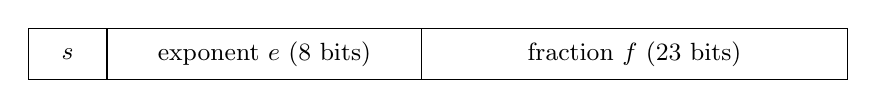
\begin{tikzpicture}[x=1cm,y=1cm]
  \draw (0,0) rectangle (1.00,0.65);
  \draw (1.00,0) rectangle (5.00,0.65);
  \draw (5.00,0) rectangle (10.4,0.65);
  \node[font=\small] at (0.50,0.325) {$s$};
  \node[font=\small] at (3.00,0.325) {exponent $e$ (8 bits)};
  \node[font=\small] at (7.70,0.325) {fraction $f$ (23 bits)};
\end{tikzpicture}
\end{center}


\noindent
For a normalized value,
\[
  fl(r)=(-1)^s2^{e-127}(1.f)_2.
\]
The bias, $b$ is $127$.

\begin{example}
Write $x=-1234$ in IEEE 754 single-precision floating-point representation and hexadecimal form.
\end{example}

\begin{solution}[6.5cm]
Converting $1234_{10}$ to binary:
\[
 1234_{10}=10011010010_2
 =1.0011010010_2\times2^{10}.
\]
Therefore
\[
 s=1,
 \qquad e=10+127=137=10001001_2.
\]
The fraction field is the part after the leading $1$:
\[
 f=00110100100000000000000.
\]
Hence the $32$ bits are
\[
 \underbrace{1}_{s}\;
 \underbrace{10001001}_{e}\;
 \underbrace{00110100100000000000000}_{f},
 \text{ or }
 11000100100110100100000000000000_2.
\]
Grouping into blocks of four gives
\[
 1100\;0100\;1001\;1010\;0100\;0000\;0000\;0000
 =\boxed{\texttt{C49A4000}}.
\]
\end{solution}

\begin{example}
Given $x=4.375_{10}=100.011_2$, convert $x$ to IEEE 754 single precision and give the answer in hexadecimal form.
\end{example}

\begin{solution}[5.5cm]
In scientific notation, we have:
\[
 100.011_2=1.00011_2\times2^2.
\]
Thus
\[
 s=0,
 \quad e=2+127=129=10000001_2,
\quad f=00011000000000000000000.
\]
The bit pattern is
\[
 0\;10000001\;00011000000000000000000.
\]
Grouping into hexadecimal digits,
\[
 0100\;0000\;1000\;1100\;0000\;0000\;0000\;0000
 =\boxed{\texttt{408C0000}}.
\]
\end{solution}

\subsection{IEEE 754 Double Precision}

A normalized double-precision number uses one sign bit, eleven exponent bits, and fifty-two fraction bits:

\begin{center}
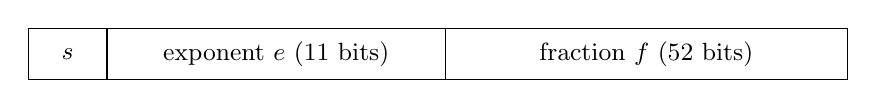
\begin{tikzpicture}[x=1cm,y=1cm]
  \draw (0,0) rectangle (1.00,0.65);
  \draw (1.00,0) rectangle (5.30,0.65);
  \draw (5.30,0) rectangle (10.4,0.65);
  \node[font=\small] at (0.50,0.325) {$s$};
  \node[font=\small] at (3.15,0.325) {exponent $e$ (11 bits)};
  \node[font=\small] at (7.85,0.325) {fraction $f$ (52 bits)};
\end{tikzpicture}
\end{center}

For a normalized value,
\[
  fl(r)=(-1)^s2^{e-1023}(1.f)_2.
\]
The bias, $b$ is $1023$.

\begin{example}
Convert the following IEEE 754 double-precision machine number to decimal:
\[
0100000000111011100100010000000000000000000000000000000000000000
\]
\end{example}

\begin{solution}[5.8cm]
Separate the fields:
\[
 s=0,
 \qquad e=10000000011_2=1027,
\]
and the fraction begins
\[
 f=1011100100010000\ldots.
\]
The true exponent is
\[
 q=e-1023=1027-1023=4.
\]
The significand is
\[
\begin{aligned}
(1.f)_2
 &=1.101110010001_2\\
 &=1+2^{-1}+2^{-3}+2^{-4}+2^{-5}+2^{-8}+2^{-12}\\
 &=1.722900390625.
\end{aligned}
\]
Therefore
\[
 r=2^4(1.722900390625)=\boxed{27.56640625}.
\]
\end{solution}

\begin{remark}
IEEE 754 also reserves exponent patterns for zero, subnormal numbers, infinities and NaN (Not a Number). The formulas above apply to normalized finite numbers.
\end{remark}

\section{Algorithms, Convergence and Accuracy}

An algorithm is a procedure that describes a finite sequence of steps performed in a specified order to solve a problem or produce a good approximation of the solution of said problem.

Many numerical algorithms are iterative. Starting from an initial approximation $x_0$, they generate a sequence
\[
    \{x_n\} = \{x_0,x_1,x_2,\ldots\}
\]
by repeatedly applying an update formula $f(x) \text{ s.t. } x_{i+1} = f(x_i)$. Main concepts are:
\begin{itemize}
  \item \textbf{initial condition}: the starting approximation or initial guess $x_0$;
  \item \textbf{iteration}: applying the algorithm $x_{i+1} = f(x_i)$;
  \item \textbf{convergence}: for a sufficiently large $N$, $x_N$ approach a limiting value;
  \item \textbf{stopping criterion}: a rule for deciding when the approximation is sufficiently accurate.
\end{itemize}

\noindent
Common stopping criteria include
\[
 |x_n-x_{n-1}|<\epsilon,
 \qquad
 \left|\frac{x_n-x_{n-1}}{x_n}\right|<\epsilon,
 \qquad
 |f(x_n)|<\epsilon,
\]
where $\epsilon$ denotes a sufficiently small error.
Sometimes, we also include a maximum allowed number of iterations.

\begin{example}
Find an approximate root of
\[
 x^2-5x+6=0.
\]
\end{example}

\begin{solution}[9.0cm]
An algorithm to estimate the root of $x^2 -5x +6 =0$ is the Newton-Raphson Method (to be covered in Chapter 3).

\noindent
We first choose an initial guess $x_0$. Let $x_0 = 0$.

\noindent
Then let
\[
 f(x)=x^2-5x+6,
 \qquad f'(x)=2x-5.
\]
Then, we improve the guess by Newton's formula:
\[
 x_{n+1}=x_n-\frac{f(x_n)}{f'(x_n)}
 =x_n-\frac{x_n^2-5x_n+6}{2x_n-5}.
\]
Repeatedly applying the formula until desirable accuracy, we have:
\[
\begin{array}{c|c}
\toprule
n & x_n\\
\midrule
0&1.000000\\
1&1.666667\\
2&1.933333\\
3&1.996078\\
4&1.999985\\
5&2.000000\\
\bottomrule
\end{array}
\]
Thus, the sequence converges to the root $x=2$.

\bigskip \noindent
Checking the exact solution, our above equation factors as:
\[
 x^2-5x+6=(x-2)(x-3),
\]
so the exact roots are $2$ and $3$.

\bigskip \noindent
Looking at our approximation and accuracy at $n=4$, the absolute error relative to the exact root is approximately
\[
 |2-x_4| = |2-1.999985|\approx1.5\times10^{-5}.
\]
A practical implementation would stop once a prescribed stopping criteria (e.g. a tolerance or error, $\epsilon$, or usually an approximation of such an error) is met, or once a given maximum iteration count is reached.
\end{solution}

\begin{remark}
Convergence is not guaranteed merely because an iterative formula can be written down. The choice of algorithm, initial approximation and stopping criterion can all affect whether the computed sequence converges and how quickly it does so.
\end{remark}

\bigskip

In the upcoming chapters, we will explore a handful of algorithms to approximate a solution to a few different types of problems.

\phantomsection
\section*{Tutorial 1}
\addcontentsline{toc}{section}{Tutorial 1}

\begin{enumerate}[
    label=\arabic*.,
    leftmargin=1.5em,
    itemsep=0.4em,
    parsep=0.1em
]

    \item Let \(f(x)=\sqrt{x+1}\).
    \begin{enumerate}[
        label=(\alph*),
        leftmargin=2em,
        itemsep=0pt,
        topsep=0.2em,
        parsep=0pt,
        partopsep=0pt
    ]
        \item Find the third-order Taylor polynomial \(P_3(x)\)
        about \(x_0=0\).
        \item Use \(P_3(x)\) to approximate
        \(\sqrt{0.5}\) and \(\sqrt{1.25}\).
        \item Find the absolute errors of the approximations in part~(b).
    \end{enumerate}

    \item Let \(f(x)=\cos x\).
    \begin{enumerate}[
        label=(\alph*),
        leftmargin=2em,
        itemsep=0pt,
        topsep=0.2em,
        parsep=0pt,
        partopsep=0pt
    ]
        \item Find the third-order Taylor polynomial \(P_3(x)\)
        for the function \(f(x)\) about \(x_0=0\).
        \item Find an upper bound for the truncation error when
        approximating \(\cos(0.01)\) using the polynomial obtained
        in part~(a).
    \end{enumerate}

    \item
    \begin{enumerate}[
        label=(\alph*),
        leftmargin=2em,
        itemsep=0pt,
        topsep=0pt,
        parsep=0pt,
        partopsep=0pt
    ]
        \item Convert the decimal number \(5432_{10}\) to a binary number.
        \item Convert the binary number
        \(1010100111000_2\) to a decimal number.
        \item Convert the binary number
        \(1010100111000_2\) to a hexadecimal number.
        \item Convert the hexadecimal number
        \(1538_{16}\) to a decimal number.
    \end{enumerate}

    \item Convert each of the following binary numbers into decimal
    and hexadecimal numbers.
    \begin{enumerate}[
        label=(\alph*),
        leftmargin=2em,
        itemsep=0pt,
        topsep=0.2em,
        parsep=0pt,
        partopsep=0pt
    ]
        \item \(110011.011010_2\)
        \item \(11100010.100111_2\)
    \end{enumerate}

    \item Convert \(\dfrac{1}{3}\) to a binary number of eight significant
    digits. Find the round-off error.

    \item Convert the decimal number \(12345_{10}\) to the IEEE~754
    single-precision floating-point format.

    \item Given that
    \[
        x=10001110011.00011_2,
    \]
    convert \(x\) to the IEEE~754 single-precision floating-point
    representation. Express the answer in hexadecimal form.

    \item Convert the machine number
    \[
        01000001101110010000000000000000
    \]
    to a decimal number.

\end{enumerate}

\chapter{Numerical Linear Algebra}

\section{Linear Systems and Direct Methods}

A system of $m$ linear equations in $n$ unknowns can be written as
\[
  A\vect{x}=\vect{b},
\]
where $A=[a_{ij}]\in\R^{m\times n}$ is the coefficient matrix,
$\vect{x}=[x_1,\ldots,x_n]^T$ is the vector of unknowns, and
$\vect{b}=[b_1,\ldots,b_m]^T$ is the right-hand side.  In this course we are mainly interested in square systems, $m=n$.

We have previously learned a few direct methods to simplify linear systems so that an exact solution can easily be found. Gaussian elimination and matrix factorisation are such methods.

\subsection{Gaussian Elimination}

Gaussian elimination transforms the augmented matrix $[A\mid \vect b]$ to row-echelon form (i.e. into an upper-triangular system), or in matrix notation $[U\mid \vect b^*]$. For a pivot in row $k$, the entries below the pivot are removed using elementary row operations as follows:
\[
 R_j-m_{jk}R_k \rightarrow R_j,
 \qquad
 m_{jk}=\frac{a_{jk}^{(k)}}{a_{kk}^{(k)}},
 \qquad j=k+1,\ldots,n.
\]
For reference, $a_{ij}^{(k)}$ refers to the element in the $i$-th row and $j$-th column while eliminating entries below the pivot in the $k$-th row.
Once an upper-triangular system $U\vect{x}=\vect{b^*}$ is obtained, backward substitution gives
\[
 x_i=\frac{1}{u_{ii}}
 \left(c_i-\sum_{j=i+1}^{n}u_{ij}x_j\right),
 \qquad i=n,n-1,\ldots,1.
\]

\begin{algorithm}[Gaussian elimination]
\begin{enumerate}
  \item Form the augmented matrix $[A\mid \vect b]$.
  \item For $k=1,\ldots,n-1$, use row operations to eliminate every entry below the pivot $a_{kk}^{(k)}$.
  \item Solve the resulting upper-triangular system by backward substitution.
\end{enumerate}
\end{algorithm}

\begin{example}
Solve the following system of equations with Gaussian elimination:
\[
\begin{array}{ccccccccc}
x_1&+&x_2&+& & &3x_4&=&4,\\
2x_1&+&x_2&-&x_3&+&x_4&=&1,\\
3x_1&-&x_2&-&x_3&+&2x_4&=&-3,\\
-x_1&+&2x_2&+&3x_3&-&x_4&=&4.
\end{array}
\]
\end{example}

\begin{solution}[8.0cm]
Form the augmented matrix:
\[
\left[
\begin{array}{rrrr|r}
1&1&0&3&4\\
2&1&-1&1&1\\
3&-1&-1&2&-3\\
-1&2&3&-1&4
\end{array}
\right].
\]
Then,
\[
\left[
\begin{array}{rrrr|r}
1&1&0&3&4\\
2&1&-1&1&1\\
3&-1&-1&2&-3\\
-1&2&3&-1&4
\end{array}
\right]
\xrightarrow[
  {\displaystyle
    \begin{array}{l}
      R_4+R_1\to R_4
    \end{array}}
]{
  \begin{array}{l}
    R_2-2R_1\to R_2\\
    R_3-3R_1\to R_3
  \end{array}
}
\left[
\begin{array}{rrrr|r}
1&1&0&3&4\\
0&-1&-1&-5&-7\\
0&-4&-1&-7&-15\\
0&3&3&2&8
\end{array}
\right]
\]
\[
    \xrightarrow[
  {\displaystyle
    \begin{array}{l}
      R_4+3R_2\to R_4
    \end{array}}
]{{\displaystyle
    \begin{array}{l}
      R_3-4R_2\to R_3
    \end{array}}
}
\left[
\begin{array}{rrrr|r}
1&1&0&3&4\\
0&-1&-1&-5&-7\\
0&0&3&13&13\\
0&0&0&-13&-13
\end{array}
\right].
\]
Backward substitution yields
\[
   x_4=\frac{-13}{-13}=1,
 \quad x_3=\frac{13-13(1)}{3}=0,
\]\[
 \quad x_2=\frac{-7+5(1)+1(0)}{-1}=2,
 \quad x_1=\frac{4-3(1)-0(0)-2}{1}=-1.
\]
Thus
\[
 \vect{x}=[-1,2,0,1]^T.
\]
\end{solution}

In most cases, Gaussian elimination is the preferred way to solve a linear system $A\vect{x}=\vect{b}$. But there are two problems with Gaussian Elimination, which we will discuss in the following subsections.

\subsection{Pivoting Strategies}

We have previously abstracted the steps for Gaussian Elimination. However, if we were to follow the steps blindly, we may run into a few problems (division by zero or numerical instabilities).

A zero pivot prevents the next elimination step (since it would cause division by zero if we were to eliminate blindly).  Even a nonzero but very small pivot can magnify round-off error because the multipliers $m_{jk}$ become large.

\begin{example}[Zero pivot]
Solve
\[
\begin{cases}
 0x_1+x_2=1 \\
 x_1+x_2=2
\end{cases}
\]
\end{example}

\begin{solution}[2.4cm]
After interchanging the two equations, the system becomes
\[
 x_1+x_2=2,
 \qquad x_2=1,
\]
and thus $x_2=1$ and $x_1=1$.
\end{solution}

\begin{example}[Small pivot]
Consider
\[
\begin{cases}
 \epsilon x_1+x_2=1\\
 x_1+x_2=2
\end{cases}
\]
where $\epsilon$ is very small.  We will see why elimination without pivoting may be unreliable.
\end{example}

\begin{solution}[3.0cm]
Using the first equation as pivot, we will perform the row operation $\displaystyle R_2-\frac{1}{\epsilon}R_1\to R_2$. Notice that the multiplier $1/\epsilon$ is very large.  The second equation becomes
\[
 \left(1-\frac1\epsilon\right)x_2
 =2-\frac1\epsilon
 \implies
 x_2 = \frac{2-\epsilon^{-1}}{1-\epsilon^{-1}}\approx 1.
\]
Substituting back into the first equation, we will get:
\[
    x_1 = \epsilon^{-1}(1-x_2) \approx \epsilon^{-1}(1-1) = 0.
\]
It is clear that this solution became unreliable when we executed Gaussian Elimination numerically. 

\noindent
(Substituting our solution $x_1 = 0, x_2 = 1$ into Equation 2 yields a contradiction.)
\end{solution}

\begin{definition}[Partial pivoting]
At a given step $k$, partial pivoting exchanges row $k$ (the original pivot row) with a row below it with the largest leading element. Mathematically, we want a row $p\ge k$ for which
\[
 |a_{pk}^{(k)}|=
 \max_{k\le i\le n}|a_{ik}^{(k)}|.
\]
Partial pivoting is applied in every step of elimination so that we can get a safe and accurate solution.
\end{definition}

\newpage
\begin{example}
Apply Gaussian elimination with partial pivoting to solve
\[
\begin{cases}
\epsilon x_1 + x_2 = 1\\
x_1 + x_2 = 2
\end{cases}
\]
when \(\epsilon\) is small.
\end{example}

\begin{solution}[3.5cm]
We see in the first column that $|1| > |\epsilon|$ which is under the pivot element. Thus exchange the two equations:
\[
\begin{cases}
 x_1+x_2=2\\
 \epsilon x_1+x_2=1
\end{cases}
\]
Then applying row operation $R_2 - \epsilon R_1 \to R_2$ gives
\[
 (1-\epsilon)x_2=1-2\epsilon,
\]
and hence
\[
 x_2=\frac{1-2\epsilon}{1-\epsilon}\approx1,
 \qquad
 x_1=2-x_2\approx1.
\]
\end{solution}

\subsection{Matrix Inversion}
If $A$ is nonsingular, its inverse can be computed by applying Gauss-Jordan elimination (i.e. reducing a matrix to r.r.e.f., reduced row-echelon form) to the block matrix $[A\mid I]$ until the left block becomes $I$:
\[
 [A\mid I]\longrightarrow[I\mid A^{-1}].
\]
However, when considering a square matrix of order $n$, finding the inverse using this method would mean applying Gauss-Jordan Elimination to an $n \times 2n$ augmented matrix.

\medskip
The issue with speed could be resolved for certain classes of problems. The table below shows the operation counts for Gaussian Elimination:
\[
\begin{array}{l|cc}
    \hline
    & \text{Multiplication/Divisions} & \text{Additions/Subtractions}\\
    \hline
    \text{Elimination Steps}& \rule{0pt}{4.0ex}\dfrac{2n^3+3n^2-5n}{6} &\rule{0pt}{4.0ex}\dfrac{n^3-n}{3} \\[1.5ex]
    \hline
    \text{Backward Substitution}& \rule{0pt}{4.0ex}\dfrac{n^2+n}{2}&\rule{0pt}{4.0ex}\dfrac{n^2-n}{2}\\[1.5ex]
    \hline
\end{array}
\]

From here, we see that the number of operations to do backward substitution is significantly smaller than doing the elimination steps.
Just considering a linear system with a $1000 \times 1000$ matrix, we would need 667,165,500 operations for elimination, but only 1,000,000 operations ($0.15\%$) to perform backward substitution.

Hence, for efficiency, when we compute the inverse for a matrix $A$, we will reduce $[A|I]$ to $[U|Y]$ where $U$ is an upper triangular matrix (or as we know the r.e.f. of $A$) and $Y$ is the matrix we get after performing the same elimination steps on $I$.
Then, we will individually obtain the columns of $A^{-1}$ through solving $U\vect{x}_i=\vect{y}_i$ where $\vect{y}_i$ denotes the $i$-th column of $Y$.

\begin{example}
Use Gaussian Elimination followed by backward substitution to find the inverse of
\[
 A=\begin{bmatrix}
 1&2&-1\\
 2&1&0\\
 -1&1&2
 \end{bmatrix}.
\]
\end{example}

\begin{solution}[5.0cm]
\[
[A|I]=
\left[\begin{array}{ccc|ccc}
1 & 2 & -1 & 1 & 0 & 0\\
2 & 1 & 0 & 0 & 1 & 0\\
-1 & 1 & 2 & 0 & 0 & 1\\
\end{array}\right]
\xrightarrow[
{\displaystyle
\begin{array}{l}
R_3+R_1\to R_3
\end{array}}]
{{\displaystyle
\begin{array}{l}
R_2-2R_1\to R_2
\end{array}}
}
\left[\begin{array}{ccc|ccc}
1 & 2 & -1 & 1 & 0 & 0\\
0 & -3 & 2 & -2 & 1 & 0\\
0 & 3 & 1 & 1 & 0 & 1
\end{array}\right]
\]
\[
\xrightarrow{\begin{array}{l}\displaystyle{R_3+R_2\to R_3}\end{array}}
\left[\begin{array}{ccc|ccc}
1 & 2 & -1 & 1 & 0 & 0 \\
0 & -3 & 2 & -2 & 1 & 0\\
0 & 0 & 3 & -1 & 1 & 1
\end{array}\right]=[U|Y]
\]
\medskip
\[
\begin{bmatrix}
1 & 2 & -1\\
0 & -3 & 2\\
0 & 0 & 3
\end{bmatrix}
\begin{bmatrix}
x_1 \\ x_2 \\ x_3
\end{bmatrix}
=
\begin{bmatrix}
1 \\ -2 \\ -1
\end{bmatrix}
\]
\[
\implies
x_3 = -\frac13, \; x_2 = \frac{-2-2(-\frac13)}{-3} = \frac49, \; x_1 = \frac{1+1(-\frac13)-2(\frac49)}{1}=-\frac29.
\]

\medskip

\[
\begin{bmatrix}
1 & 2 & -1\\
0 & -3 & 2\\
0 & 0 & 3
\end{bmatrix}
\begin{bmatrix}
x_1 \\ x_2 \\ x_3
\end{bmatrix}
=
\begin{bmatrix}
0 \\ 1 \\ 1
\end{bmatrix}
\]
\[
\implies
x_3 = \frac13, \; x_2 = \frac{1-2(\frac13)}{-3} = -\frac19, \; x_1 = \frac{0+1(\frac13)-2(-\frac19)}{1}=\frac59.
\]

\medskip

\[
\begin{bmatrix}
1 & 2 & -1\\
0 & -3 & 2\\
0 & 0 & 3
\end{bmatrix}
\begin{bmatrix}
x_1 \\ x_2 \\ x_3
\end{bmatrix}
=
\begin{bmatrix}
0 \\ 0 \\ 1
\end{bmatrix}
\]
\[
\implies
x_3 = \frac13, \; x_2 = \frac{0-2(\frac13)}{-3} = \frac29, \; x_1 = \frac{0+1(\frac13)-2(\frac29)}{1}=-\frac19.
\]

\medskip
\(
 \therefore A^{-1}=\begin{bmatrix}
 -\dfrac29&\phantom{-}\dfrac59&-\dfrac19\\[3mm]
 \phantom{-}\dfrac49&-\dfrac19&\phantom{-}\dfrac29\\[3mm]
 -\dfrac13&\phantom{-}\dfrac13&\phantom{-}\dfrac13
 \end{bmatrix}.
\)
\end{solution}

\subsection{Matrix Factorisation}
Gaussian elimination is the principal tool in the direct solution of linear system of equations. Previously, we have learnt that the steps used for elimination can also be used to factor a matrix.
Suppose the matrix \(A\) can be factorized as $A=LU$,
where $L$ is lower triangular and $U$ is upper triangular.  Then
\[
 A\vect{x}=\vect b
 \quad\Longleftrightarrow\quad
 (LU)\vect{x}=\vect b
 \quad\Longleftrightarrow\quad
 L(U\vect{x})=\vect b.
\]
Let $U\vect{x}=\vect y$.  Now the problem $A\vect x = \vect b$ has been separated into two equations $L\vect y = \vect b \text{ and } U\vect x = \vect y$. Since both $L$ and $U$ are triangular, both equations could be solved by substitution operations (forward and backward substitution respectively).

Since substitution has the operation count $\sim O(n^2)$, it is expected to speed up the process of solving $A\vect x = \vect b$. However, for only one value for $\vect b$, matrix factorization does not have much advantage over naive Gaussian Elimination. But, for different values of $\vect{b}_i$, matrix factorization would be preferred as one only needs to factorize $A$ once and the same $L$ and $U$ could be applied to the different values of $\vect{b}_i$ repeatedly.
\begin{example}
Factorise
\[
 A=\begin{bmatrix}
 1&1&0&3\\
 2&1&-1&1\\
 3&-1&-1&2\\
 -1&2&3&-1
 \end{bmatrix}
\]
into $LU$ form and solve $A\vect{x}=\vect b$ for
$\vect b=[1,1,-3,4]^T$.
\end{example}

\begin{solution}[8.0cm]
\[
A=\begin{bmatrix}
1 & 1 & 0 & 3\\
2 & 1 & -1 & 1\\
3 & -1 & -1 & 2\\
-1 & 2 & 3 & -1
\end{bmatrix}
\xrightarrow[
{\displaystyle
\begin{array}{l}
R_4+R_1\to R_4
\end{array}}]
{{\displaystyle
\begin{array}{l}
R_2-2R_1\to R_2\\
R_3-3R_1\to R_3
\end{array}}
}
\begin{bmatrix}
1 & 1 & 0 & 3\\
0 & -1 & -1 & -5\\
0 & -4 & -1 & -7\\
0 & 3 & 3 & 2
\end{bmatrix}
\xrightarrow[
{\displaystyle
\begin{array}{l}
R_4+3R_2\to R_4
\end{array}}]
{\displaystyle
\begin{array}{l}
R_3-4R_2\to R_3
\end{array}}
\]
\[
\begin{bmatrix}
1 & 1 & 0 & 3\\
0 & -1 & -1 & -5\\
0 & 0 & 3 & 13\\
0 & 0 & 0 & -13
\end{bmatrix}
=U,
\qquad
L=\begin{bmatrix}
1 & 0 & 0 & 0\\
2 & 1 & 0 & 0\\
3 & 4 & 1 & 0\\
-1 & -3 & 0 &1
\end{bmatrix}
\]
\(\therefore A\vect x = \vect b \implies LU\vect x = \vect b.\)

\noindent
Let $\vect y = U\vect x$. Then $LU\vect x = \vect b \implies L\vect y = \vect b$.
\[
\implies
\begin{bmatrix}
1 & 0 & 0 & 0\\
2 & 1 & 0 & 0\\
3 & 4 & 1 & 0\\
-1 & -3 & 0 & 1\\
\end{bmatrix}
\begin{bmatrix}
y_1 \\ y_2 \\ y_3 \\ y_4
\end{bmatrix}
=
\begin{bmatrix}
1 \\ 1 \\ -3 \\ 4
\end{bmatrix}
\implies
 y_1=1,
 \quad y_2=1-2(1)=-1,
\]
\[
 \quad y_3=-3-3(1)-4(-1)=-2,
 \quad y_4=4+1+3(-1)+0=2.
\]
\(
\implies U\vect x = \vect y \implies
\begin{bmatrix}
1 & 1 & 0 & 3\\
0 & -1 & -1 & -5\\
0 & 0 & 3 & 13\\
0 & 0 & 0 & -13\\
\end{bmatrix}
\begin{bmatrix}
x_1 \\ x_2 \\ x_3 \\ x_4
\end{bmatrix}
=
\begin{bmatrix}
1 \\ -1 \\ -2 \\ 2
\end{bmatrix}
\)

\smallskip
\noindent
\(\displaystyle
\implies
 x_4=-\frac2{13},
 \quad x_3=-2-13\left(-\frac{2}{13}\right)=0,
 \quad x_2=\frac1{-1}\left(-1+5\left(-\frac2{13}\right)+0\right)=\frac{23}{13},
\)

\smallskip
\noindent
\(\displaystyle
\; \; \qquad x_1=1-3\left(-\frac2{13}\right)-0-\frac{23}{13}=-\frac4{13}.
\)

\[
 \therefore \vect x=\left[-\frac4{13},\frac{23}{13},0,-\frac2{13}\right]^T.
\]
\end{solution}

\section{Iterative Methods for Solving Linear Systems}

In this section, iterative methods start with an initial guess or approximation to a solution, $\vect{x}^{(0)}$ and then generate a succession of better and better approximations
\[
 \vect{x}^{(1)},\vect{x}^{(2)},\vect{x}^{(3)},\ldots
\]
that (may) tend toward the exact solution.
We will discuss three iterative methods:
\begin{enumerate}
\item Jacobi method
\item Gauss-Seidel method
\item Successive Over-relaxation (SOR) method
\end{enumerate}

\noindent
To get the idea, we separate our coefficient matrix A from our linear system as the following:
\[
 A=D+L+U,
\]
where $D$ contains the diagonal entries of $A$, $L$ the entries below the diagonal, and $U$ the entries above the diagonal.

\noindent
Don't worry if the formulas found in the explanations below feel a bit overwhelming. For first time learners, referring to the example to get a feel how the methods work will clear up a lot of the confusion. The same goes for the majority of sections that follow in future chapters. The formulas are just there to properly define how the methods work in mathematical terms (that may be useful when trying to implement the methods in programming).

\subsection{Jacobi Method}
Consider a linear system with $n$ equations and $n$ unknowns. Then we first solve for $x_i$ in the $i$-th equation (where $i=1,2,\dots,n$) to derive our iteration equation.
Componentwise,
\[
 x_i^{(k+1)}
 =\frac{1}{a_{ii}}
 \left(b_i-\sum_{j\ne i}a_{ij}x_j^{(k)}\right).
\]
In matrix notation, the Jacobi iteration is
\[
 \vect{x}^{(k+1)}
 =D^{-1}\bigl(\vect b-(L+U)\vect{x}^{(k)}\bigr).
\]
The order in which the equations are examined is irrelevant, since the Jacobi method treats them independently. That is, we prepare the vector $\vect x^{(k+1)}$ only using $\vect x^{(k)}$, or iterating in batches, only with the information from the previous iteration. For this reason, the Jacobi method is also known as the \textbf{method of simultaneous corrections}, since the updates could in principle be done simultaneously.

\subsection{Gauss--Seidel Method}
Similar to the Jacobi method, we prepare the iteration equations by solving for $x_i$ in the $i$-th equation of our linear system. Componentwise,
\[
 x_i^{(k+1)}=\frac{1}{a_{ii}}
 \left(
 b_i-\sum_{j<i}a_{ij}x_j^{(k+1)}
     -\sum_{j>i}a_{ij}x_j^{(k)}
 \right).
\]
In matrix notation, the Gauss--Seidel iteration is
\[
 (D+L)\vect{x}^{(k+1)}
 =\vect b-U\vect{x}^{(k)}.
\]
Unlike the Jacobi method where $\vect x^{(k)}$ is prepared in batches, each element of $\vect x^{(k)}$, $x^{(k)}_i$ depends on $x^{(k)}_j \; \forall j<i$; that is we iterate with the \textbf{latest information} instead of information from the previous iteration. 
This is a \textbf{method of successive corrections}; it \textbf{replaces approximations by corresponding new ones} as soon as the latter are available.
Note that since newly computed values are used immediately, so Gauss--Seidel often converges faster than Jacobi.

\subsection{Successive Over-Relaxation}
Modification of the Gauss-Seidel method with the relaxation parameter $\omega \; (0<\omega<2)$ is done to improve the rate of convergence. Componentwise, we only add weights as follows:
\[
 x_i^{(k+1)}
 =
 \frac{\omega}{a_{ii}}
 \left(
 b_i-\sum_{j<i}a_{ij}x_j^{(k+1)}
     -\sum_{j>i}a_{ij}x_j^{(k)}
 \right)+(1-\omega)x_i^{(k)},
\qquad 0<\omega<2.
\]
\begin{itemize}
\item If $\omega=1$, SOR reduces to Gauss--Seidel.
\item Values $0<\omega<1$ under-relax the iteration, which might help to dampen the iteration to achieve convergence if the Gauss-Seidel method diverges.
\item Meanwhile, if the Gauss-Seidel already converges, values $1<\omega<2$ will help to speed up the convergence by over-relaxation.
\end{itemize}

\begin{definition}[Strict diagonal dominance]
A square matrix $A=[a_{ij}]$ of order $n$ is strictly diagonally dominant if
\[
 |a_{kk}| >\sum_{\substack{i=1\\ i\ne k}}^{n}|a_{ki}|,
 \qquad k=1,2,\ldots,n.
\]
That is, A is strictly diagonally dominant if the absolute value of each diagonal entry is greater than the sum of the absolute values of the remaining entries in the same row.
\end{definition}

\begin{example}
Show that
\(
 A=\begin{bmatrix}
 2&-7&4\\
 8&1&6\\
 -3&5&9
 \end{bmatrix}
\)
is not strictly diagonally dominant.
\end{example}

\begin{solution}[2.5cm]
We see from the first and second row that
\(
 |2|<|-7|+|4|=11
\)
and $|1|<|8|+|6|=14$. 
Hence, $A$ is not strictly diagonally dominant.
\end{solution}

\begin{theorem}[Convergence of the Iterative Methods]
If a square matrix $A$ is strictly diagonally dominant, then the Jacobi and Gauss--Seidel approximations to the solution of the linear system $A\vect x = \vect b$ both converge to the exact solution for all choices of the initial approximation or guess, $\vect{x}^{(0)}$.
\end{theorem}

\noindent
Before we finally demonstrate how to execute these iterative methods in practice, we need to define a termination criterion. For these methods in this course, we commonly stop the computation when
\[
    \max_i|x_i^{(k+1)}-x_i^{(k)}|<\epsilon, 
    \quad \text{where } \epsilon \text{ is the pre-specified stopping criterion}.
\]
In practice however, a residual test such as $\norm{\vect b-A\vect{x}^{(k)}}<\epsilon$ may also be considered because it measures how well the computed vector satisfies the original equations.

\begin{example}
Use the \textbf{Jacobi method}, to solve
\[
\begin{aligned}
20x_1+x_2-x_3&=17\\
x_1-10x_2+x_3&=13\\
-x_1+x_2+10x_3&=18
\end{aligned}
\]
Iterate until $|x_i^{[p+1]}-x_i^{[p]}| < 0.0002$, for all $i$. Prepare all the computations in 5 decimal places.
\end{example}

\begin{solution}[8.0cm]
\[
 x_1^{[k+1]}=\frac{17-x_2^{[k]}+x_3^{[k]}}{20},
 \quad
 x_2^{[k+1]}=\frac{13-x_1^{[k]}-x_3^{[k]}}{-10},
 \quad
 x_3^{[k+1]}=\frac{18+x_1^{[k]}-x_2^{[k]}}{10}.
\]
Let our initial guess be: $x_1^{[0]}=x_2^{[0]}=x_3^{[0]}=0$. Then

\smallskip
\(\displaystyle
x_1^{[1]}=\frac{17}{20}=0.85000, \quad x_2^{[1]}=-\frac{13}{10}=-1.30000, \quad x_3^{[1]}=\frac{18}{10}=1.80000.
\)

\smallskip
\(
|x_1^{[1]} - x_1^{[0]}| = |0.85000-0| = 0.85 \geq 0.0002.
\)

\bigskip
\(\displaystyle
x_1^{[2]}=\frac{17-(-1.3)+1.8}{20}=1.00500, \quad x_2^{[2]}=-\frac{13-0.85-1.8}{10}=-1.03500,\)

\smallskip
\(\displaystyle x_3^{[2]}=\frac{18+0.85-(-1.3)}{10}=2.01500.
\)

\smallskip\(
|x_1^{[2]} - x_1^{[1]}| = |1.00500-0.85000| = 0.15500 \geq 0.0002.
\)

\bigskip
\(\displaystyle
x_1^{[3]}=\frac{17-(-1.035)+2.015}{20}=1.00250, \quad x_2^{[3]}=-\frac{13-1.005-2.015}{10}=-0.99800,\)

\smallskip
\(\displaystyle x_3^{[3]}=\frac{18+1.005-(-1.035)}{10}=2.00400.
\)

\smallskip\(
|x_1^{[3]} - x_1^{[2]}| = |1.00250-1.00500| = 0.0025 \geq 0.0002.
\)

\bigskip
\(\displaystyle
x_1^{[4]}=\frac{17-(-0.998)+2.004}{20}=1.00010, \quad x_2^{[4]}=-\frac{13-1.0025-2.004}{10}=-0.99935,\)

\smallskip
\(\displaystyle x_3^{[4]}=\frac{18+1.0025-(-0.998)}{10}=2.00005.
\)

\smallskip\(
|x_1^{[4]} - x_1^{[3]}| = |1.00010-1.00250| = 0.00240 \geq 0.0002.
\)

\bigskip
\(\displaystyle
x_1^{[5]}=\frac{17-(-0.99935)+2.00005}{20}=0.99997, \)

\smallskip
\(\displaystyle x_2^{[5]}=-\frac{13-1.0001-2.00005}{10}=-0.99999,\)

\smallskip
\(\displaystyle x_3^{[5]}=\frac{18+1.00010-(-0.99935)}{10}=1.99994.
\)

\smallskip\(
|x_1^{[5]} - x_1^{[4]}| = |0.99997-1.00010| = 0.00013 < 0.0002.
\)

\smallskip\(
|x_2^{[5]} - x_2^{[4]}| = |-0.99998-(-0.99935)| = 0.00063 \geq 0.0002.
\)

\bigskip
\(\displaystyle
x_1^{[6]}=\frac{17-(-0.99999)+1.99994}{20}=1.00000, \)

\smallskip
\(\displaystyle x_2^{[6]}=-\frac{13-0.99997-1.99994}{10}=-1.00000,\)

\smallskip
\(\displaystyle x_3^{[6]}=\frac{18+0.99997-(-0.99999)}{10}=2.00000.
\)

\smallskip\(
|x_1^{[6]} - x_1^{[5]}| = |1.00000-0.99997| = 0.00003 < 0.0002.
\)

\smallskip\(
|x_2^{[6]} - x_2^{[5]}| = |-1-(-0.99998)| = 0.00002 < 0.0002.
\)

\smallskip\(
|x_3^{[6]} - x_3^{[5]}| = |2.00000-1.99994| = 0.00006 < 0.0002.
\)

\medskip
\noindent
Hence, $x_1 = 1, x_2 = -1, x_3 =2$.
\end{solution}

\begin{example}
Redo the previous example but by using the Gauss--Seidel method.
\end{example}

\begin{solution}[6.5cm]
\[
 x_1^{[k+1]}=\frac{17-x_2^{[k]}+x_3^{[k]}}{20},
 \quad
 x_2^{[k+1]}=\frac{13-x_1^{[k+1]}-x_3^{[k]}}{-10},
 \quad
 x_3^{[k+1]}=\frac{18+x_1^{[k+1]}-x_2^{[k+1]}}{10}.
\]
Let our initial guess be: $x_1^{[0]}=x_2^{[0]}=x_3^{[0]}=0$. Then

\smallskip
\(\displaystyle
x_1^{[1]}=\frac{17}{20}=0.85000, \quad x_2^{[1]}=-\frac{13-0.85}{10}=-1.21500, \)

\smallskip
\(\displaystyle x_3^{[1]}=\frac{18+0.85-(-1.215)}{10}=2.00650.\)

\smallskip
\(
|x_1^{[1]} - x_1^{[0]}| = |0.85000-0| = 0.85 \geq 0.0002.
\)

\bigskip
\(\displaystyle
x_1^{[2]}=\frac{17-(-1.215)+2.0065}{20}=1.01108, \quad x_2^{[2]}=-\frac{13-1.01108-2.0065}{10}=-0.99824,\)

\smallskip
\(\displaystyle x_3^{[2]}=\frac{18+1.01108-(-0.99824)}{10}=2.00093.
\)

\smallskip\(
|x_1^{[2]} - x_1^{[1]}| = |1.01108-0.85000| = 0.16108 \geq 0.0002.
\)

\bigskip
\(\displaystyle
x_1^{[3]}=\frac{17-(-0.99824)+2.00093}{20}=0.99996, \)

\smallskip
\(\displaystyle x_2^{[3]}=-\frac{13-0.99996-2.00093}{10}=-0.99991,\)

\smallskip
\(\displaystyle x_3^{[3]}=\frac{18+0.99996-(-0.99991)}{10}=1.99999
\)

\smallskip\(
|x_1^{[3]} - x_1^{[2]}| = |1.01108-0.99996| = 0.01112 \geq 0.0002.
\)

\bigskip
\(\displaystyle
x_1^{[4]}=\frac{17-(-0.99991)+1.99999}{20}=1.00000, \quad x_2^{[4]}=-\frac{13-1-1.99999}{10}=-1.00000,\)

\smallskip
\(\displaystyle x_3^{[4]}=\frac{18+1-(-1)}{10}=2.00000.
\)

\smallskip\(
|x_1^{[4]} - x_1^{[3]}| = |1.00000-0.99996| = 0.00004 < 0.0002.
\)

\smallskip\(
|x_2^{[4]} - x_2^{[3]}| = |-1.00000-(-0.99991)| = 0.00009 < 0.0002.
\)

\smallskip\(
|x_3^{[4]} - x_3^{[3]}| = |2.00000-1.99999| = 0.00001 < 0.0002.
\)

%\[
%\begin{array}{c|rrr}
%\toprule
%k&x_1^{(k)}&x_2^{(k)}&x_3^{(k)}\\
%\midrule
%0&0&0&0\\
%1&0.85000&-1.21500&2.00650\\
%\midrule
%2&1.01108&-0.99824&2.00093\\
%3&0.99996&-0.99991&1.99999\\
%4&0.99999&-1.00000&2.00000\\
%\bottomrule
%\end{array}
%\]
\medskip \noindent
Hence, $x_1 = 1, x_2 = -1, x_3 = 2$.
\end{solution}

\begin{example}
Use two iterations of \textbf{Successive Over-relaxation (SOR) method} to solve
\[
\begin{aligned}
3x_1-x_2+x_3&=-1,\\
-x_1+3x_2-x_3&=7,\\
x_1-x_2+3x_3&=-7.
\end{aligned}
\]
with $\omega = 1.25$ and initial approximation $x_1^{[0]}=0,x_2^{[0]}=0,x_3^{[0]}=0$.
\end{example}

\begin{solution}[5.5cm]
With $\omega=1.25$, we have:

\smallskip
\noindent
\(\displaystyle
x_1^{[k+1]}=\frac{1.25}{3}(-1+x_2^{[k]}-x_3^{[k]})-0.25x_1^{[k]}, 
\quad x_2^{[k+1]}=\frac{1.25}{3}(7+x_1^{[k+1]}+x_3^{[k]})-0.25x_2^{[k]},
\)

\smallskip \noindent
\(\displaystyle x_3^{[k+1]}=\frac{1.25}{3}(-7-x_1^{[k+1]}+x_2^{[k+1]})-0.25x_3^{[k]}.\)

\noindent Then

\smallskip
\(\displaystyle
x_1^{[1]}=\frac{1.25}{3}(-1)-0=-0.4167, \quad x_2^{[1]}=\frac{1.25}{3}(7-0.4167)-0=2.7431,
\)

\smallskip
\(\displaystyle
x_3^{[1]}=\frac{1.25}{3}(-7-(-0.4167)+2.7431)-0=-1.6001.
\)

\bigskip
\(\displaystyle
x_1^{[2]}=\frac{1.25}{3}(-1+2.7431-(-1.6001))-0.25(-0.4167)=1.4972, \)

\smallskip
\(\displaystyle x_2^{[2]}=\frac{1.25}{3}(7+1.4972-1.6001)-0.25(2.7431)=2.1880,
\)

\smallskip
\(\displaystyle
x_1^{[3]}=\frac{1.25}{3}(-7-1.4972+2.1880)-0.25(-1.6001)=-2.2288.
\)

\medskip \noindent
Hence, $x_1 = 1.4972, x_2 = 2.188, x_3 = -2.2288$.
\end{solution}

\subsection{Conjugate Gradient Method}
The Conjugate Gradient Method is a popular iterative method for solving a sparse system. Consider a quadratic form and its gradient:
\[
f(\vect x) = \frac12 \vect x^TA \vect x - \vect x^T \vect b,
\qquad \nabla f(\vect x) = \frac12 (A^T\vect x + A\vect x) - \vect b.
\]
If $A$ is symmetric, then $\nabla f(\vect x) = A\vect x - \vect b$.
Therefore, $f(\vect x)$ has a critical point at $\vect x$ if $A\vect x = \vect b$. Thus, if $A$ is a positive, definite, and symmetric, then we can solve $A\vect x = \vect b$ by minimising $f(x)$.

In Machine Learning, the method of steepest descent (or more widely known as gradient descent) is an another algorithm used to minimise a loss function $f(\vect x)$. 
But it converges much more slowly towards to exact solution.
On the other hand, the conjugate gradient method is able to reach the \textbf{exact solution} in at most $\mathbf{n}$ steps (given $A$ is a square matrix of order $n$).
\textbf{This section will be rewritten in the future due to having too many gaps in understanding.}
%On the other hand, the conjugate gradient method constructs mutually $A$-conjugate search directions and, in exact arithmetic, reaches the exact solution in at most $n$ steps.

\begin{algorithm}[Conjugate gradient]
Start with an initial approximation $\vect{x}_0$. Then
\[
 1.\;\vect r_0=\vect b-A\vect{x}_0,
 \qquad
 2.\;\mathbf{P}_0=\vect r_0.
\]
For $k=0,1,2,\ldots,n$, compute
\[
 \alpha_k=\frac{\vect r_k\T\vect r_k}{\vect p_k\T A\vect p_k},
 \qquad
 \vect{x}_{k+1}=\vect{x}_k+\alpha_k\vect p_k,
\]
\[
 \vect r_{k+1}=\vect r_k-\alpha_kA\vect p_k,
 \qquad
 \beta_k=\frac{\vect r_{k+1}\T\vect r_{k+1}}{\vect r_k\T\vect r_k},
\]
\[
 \vect p_{k+1}=\vect r_{k+1}+\beta_k\vect p_k.
\]
\end{algorithm}

\begin{example}
Apply conjugate gradient with $\vect{x}_0=\vect0$ to
\[
 A=\begin{pmatrix}
4&3&0\\3&4&-1\\0&-1&4
\end{pmatrix},
\qquad
\vect b=\begin{pmatrix}24\\30\\-24\end{pmatrix}.
\]
\end{example}

\begin{solution}[7.0cm]
The successive approximations are
\[
\begin{array}{c|rrr}
\toprule
k&x_1&x_2&x_3\\
\midrule
0&0&0&0\\
1&3.52577&4.40722&-3.52577\\
2&2.85801&4.14897&-4.95422\\
3&3.00000&4.00000&-5.00000\\
\bottomrule
\end{array}
\]
The residual after the third step is zero to round-off accuracy, giving
\[
 \vect{x}=(3,4,-5)\T.
\]
\end{solution}

\section{Eigenvalues and Eigenvectors}

\begin{definition}[Eigenvalues and Eigenvectors]
A scalar $\lambda$ is an eigenvalue of an $n\times n$ matrix $A$ if there exists a nonzero vector $\vect v \in \mathbb{R}^n$ such that
\[
 A\vect v=\lambda\vect v.
\]
The nonzero vector $\vect v$ is an eigenvector corresponding to $\lambda$.
\end{definition}

\noindent
Note that eigenvalues satisfy the characteristic equation
\(
 \det(A-\lambda I)=0.
\)
Once $\lambda$ is known, its corresponding eigenvectors are the nonzero solutions of
$(A-\lambda I)\vect v=\vect0$.

\begin{example}
For
\[
 A=\begin{bmatrix}4&1\\3&2\end{bmatrix},
 \qquad
 \vect v=\begin{bmatrix}1\\1\end{bmatrix},
\]
verify that $\vect v$ is an eigenvector of $A$ and find its corresponding eigenvalue.
\end{example}

\begin{solution}[2.2cm]
\[
 A\vect v
 =\begin{bmatrix}4&1\\3&2\end{bmatrix}\begin{bmatrix}1\\1\end{bmatrix}
 =\begin{bmatrix}5\\5\end{bmatrix}
 =5\begin{bmatrix}1\\1\end{bmatrix}.
\]
Hence $\vect v$ is an eigenvector corresponding to $\lambda=5$.
\end{solution}

\subsection{Gerschgorin Discs}

\begin{theorem}[Gercshgorin's theorem]
The eigenvalues of an $n\times n$ matrix $A$ lie in the union of $n$ discs
\[
 \abs{\lambda-a_{ii}}\le r_i,
 \quad
 r_i=\sum_{j\ne i}|a_{ij}| = |a_{i1}| + \dots + |a_{i,i-1}| + |a_{i,i+1}| + \dots + |a_{in}|.
\]
\end{theorem}

Gerschgorin's Theorem (or Gershgorin's Theorem) is a finding that is common taught in Complex Analysis that is used to estimate the location of the eigenvalues of a matrix $A$. For a general square matrix, the union of the $n$ disks would be drawn as circles on the complex plane. However, for a real symmetric matrix, all eigenvalues are real, so the discs may be viewed as intervals on the real line.

\begin{example}
Find Gerschgorin intervals corresponding to
\[
 A=\begin{bmatrix}
7&4&-4\\
4&-8&-1\\
-4&-1&-8
\end{bmatrix}.
\]
\end{example}

\begin{solution}[3.8cm]
The row radii are
\[
 r_1=|4|+|-4|=8,
 \qquad r_2=|4|+|-1|=5,
 \qquad r_3=|-4|+|-1|=5.
\]
Thus we have
\[
|\lambda_1 - 7| \leq 8 \implies -8+7 \leq \lambda_1 \leq 8+1 \implies -1 \leq \lambda_1 \leq 15.
\]
\[
|\lambda_2 - (-8)| \leq 5 \implies -5-8 \leq \lambda_1 \leq -5+8 \implies -13 \leq \lambda_2 \leq -3.
\]
\[
|\lambda_3 - (-8)| \leq 5 \implies -5-8 \leq \lambda_3 \leq -5+8 \implies -13 \leq \lambda_3 \leq -3.
\]

\(\displaystyle \therefore \text{The eigenvalues of A, } \lambda \in [-13, -3] \cup [-1,15]\).
\end{solution}

\subsection{Power Method}

\begin{definition}[Dominant eigenvalue]
An eigenvalue $\lambda_1$ is dominant if
\[
 |\lambda_1|>|\lambda_j|
 \qquad\text{for every }j\ne1.
\]
That is if the absolute value of $\lambda$ is larger than the absolute values of all the other remaining eigenvalues. An eigenvector corresponding to the dominant eigenvalue is thus also called a dominant eigenvector.
\end{definition}

\begin{example}
We explore the concept of dominant eigenvalues in the following cases:
\begin{enumerate}[label=(\alph*),leftmargin=2.7em]
\item A $4\times 4$ matrix A with eigenvalues $\lambda=-5,4,2,-3$ has dominant eigenvalue $\lambda = -5$ since 
\[\lvert -5\rvert > \lvert 4\rvert,\quad
\lvert -5\rvert > \lvert 2\rvert,\quad
\lvert -5\rvert > \lvert -3\rvert.\]
\item A $3\times 3$ matrix $A$ with eigenvalues $\lambda=2,-5,5$ has no dominant eigenvalue since \[\lvert -5 \rvert \ngtr \lvert 5 \rvert.\]
\end{enumerate}
\end{example}

\begin{theorem}[The Power Method or Direct Iteration Method]
If an $n\times n$ matrix $A$ is diagonalizable (i.e. having $n$ distinct eigenvalues) and the initial guess for the dominant eigenvector $\vect v$, $\vect x_0$ has a nonzero component in the dominant eigendirection, then
\[
\vect x_k = A^k\vect{x}_0 = A \vect x_{k-1}
\]
is a good approximation to a dominant eigenvector when $k$ is sufficiently large.
\end{theorem}

\begin{enumerate}[label=(\alph*)]
\item The dominant eigenvalue may be approximated using the current approximation to the dominant eigenvector $\vect x_k = A^k\vect x_0$ by the \textbf{Rayleigh quotient}
\[
\lambda \approx \frac{\vect{x}_k^T A\vect{x}_k}{\vect{x}_k^T\vect{x}_k} = \frac{A\vect x_k \cdot \vect x_k}{\vect x_k \cdot \vect x_k}.
\]
\item The \textbf{convergence rate} depends on the ratios of the other remaining eigenvectors to the dominant eigenvector
\[
\frac{\lambda_2}{\lambda}, \dots , \frac{\lambda_n}{\lambda}.
\]
The smaller the ratios, the faster the rate of convergence.
\end{enumerate}


\begin{example}
Let
\[
 A=\begin{bmatrix}4&-2\\3&-1\end{bmatrix},
 \qquad
 \vect{x}_0=\begin{bmatrix}1\\0\end{bmatrix}.
\]
Use the power method to approximate the dominant eigenvalue and a corresponding eigenvector with the initial guess given above. Prepare 6 iterations.
\end{example}

\begin{solution}[6.8cm]
\(\vect{x}_1=A\vect x_0 = \begin{bmatrix}4&-2\\3&-1\end{bmatrix}
\begin{bmatrix}1\\0\end{bmatrix}=\begin{bmatrix}4\\3\end{bmatrix}\)

\smallskip \noindent
\(\vect{x}_2=\begin{bmatrix}4&-2\\3&-1\end{bmatrix}\begin{bmatrix}4\\3\end{bmatrix}
=\begin{bmatrix}10\\9\end{bmatrix}\)

\smallskip \noindent
\(\vect{x}_3=\begin{bmatrix}4&-2\\3&-1\end{bmatrix}\begin{bmatrix}10\\9\end{bmatrix}
=\begin{bmatrix}22\\21\end{bmatrix}\)

\smallskip \noindent
\(\vect{x}_4=\begin{bmatrix}4&-2\\3&-1\end{bmatrix}\begin{bmatrix}22\\21\end{bmatrix}
=\begin{bmatrix}46\\45\end{bmatrix}\)

\smallskip \noindent
\(\vect{x}_5=\begin{bmatrix}4&-2\\3&-1\end{bmatrix}\begin{bmatrix}46\\45\end{bmatrix}
=\begin{bmatrix}94\\93\end{bmatrix}\)

\smallskip \noindent
\(\vect{x}_6=\begin{bmatrix}4&-2\\3&-1\end{bmatrix}\begin{bmatrix}94\\93\end{bmatrix}
=\begin{bmatrix}190\\189\end{bmatrix}\)

\begin{flalign*}
\therefore \text{The dominant eigenvalue, }\lambda
&\approx
\frac{\mathbf{x}_6^T A\mathbf{x}_6}
     {\mathbf{x}_6^T\mathbf{x}_6}=
\frac{
\begin{bmatrix}190\\189\end{bmatrix}^{T}
\begin{bmatrix}4&-2\\3&-1\end{bmatrix}
\begin{bmatrix}190\\189\end{bmatrix}
}{
\begin{bmatrix}190\\189\end{bmatrix}^{T}
\begin{bmatrix}190\\189\end{bmatrix}
}
=
\frac{
\begin{bmatrix}190&189\end{bmatrix}
\begin{bmatrix}382\\381\end{bmatrix}
}{
190^2+189^2
} &&\\[4pt]
&=
\frac{190(382)+189(381)}
     {190^2+189^2}
=2.0132. &&
\end{flalign*}
\end{solution}

\noindent
We can observe some key facts from the previous example:
\begin{enumerate}
\item It is clear that the vectors $x_m$ are getting closer and closer to scalar multiples of
    $\begin{bmatrix}1\\1\end{bmatrix}$ which is a dominant eigenvector of $A$. By checking, we also see that the corresponding dominant eigenvalue, $\lambda = 2$.
\item The convergence is rather slow.
\item The power method often generates a sequence of vectors $\{A^k\vect x_0\}$ that have inconveniently large entries.
\end{enumerate}

\begin{theorem}[Power Method with Scaling]
The large entries discussed earlier can be avoided by scaling the iterative vector at each step. 

\smallskip
\noindent
That is, we first compute
\(\displaystyle
\vect y_{k} = A\vect{x}_{k-1} = [y_1, \dots, y_n]^T \text{ and multiply it by }
\frac1{ \max \{|y_{1}|,\dots,|y_{n}|\}}\) to get
\[
    \vect x_{k+1} = \frac1{\max\{|A\vect x_k|\}}A\vect x_{k}.
\]
\end{theorem}
We repeat this process to obtain scaled-down vectors, and the approximate dominant eigenvalue (at step $k$) is computed using the Rayleigh quotient:
\[
\lambda (k) = \frac{\vect x_k^T A \vect x_k}{\vect x_k^T \vect x_k} = \frac{A\vect x_k \cdot \vect x_k}{\vect x_k \cdot \vect x_k}.
\]
We will \textbf{STOP} the computation at the $k$-th step if the \textbf{estimated relative error} or \textbf{estimated percentage error} is low enough:
\[
\left| \frac{\lambda(k)-\lambda(k-1)}{\lambda(k)} \right| < \epsilon, \quad
\text{ or } \quad \left| \frac{\lambda(k)-\lambda(k-1)}{\lambda(k)} \right| < \epsilon, \quad
\text{ for a small } \epsilon.
\]

\begin{example}
Repeat the previous example using power iteration with scaling.
\end{example}

\begin{solution}[3.6cm]
\(\displaystyle
A\vect x_0 = \begin{bmatrix}4&-2\\3&-1\end{bmatrix}
\begin{bmatrix}1\\0\end{bmatrix}=\begin{bmatrix}4\\3\end{bmatrix},
\quad \vect x_1 = \frac14 \begin{bmatrix}4\\3\end{bmatrix}=\begin{bmatrix}1\\0.75\end{bmatrix}\)

\smallskip \noindent
\(\displaystyle
A\vect x_1=\begin{bmatrix}4&-2\\3&-1\end{bmatrix}\begin{bmatrix}1\\0.75\end{bmatrix}
=\begin{bmatrix}2.5\\2.25\end{bmatrix},
\quad \vect x_2 = \frac1{2.5}\begin{bmatrix}2.5\\2.25\end{bmatrix} = \begin{bmatrix}1\\0.9\end{bmatrix}\)

\smallskip \noindent
\(\displaystyle
A\vect x_2=\begin{bmatrix}4&-2\\3&-1\end{bmatrix}\begin{bmatrix}1\\0.9\end{bmatrix}
=\begin{bmatrix}2.2\\2.1\end{bmatrix},
\quad \vect x_3 = \frac1{2.2}\begin{bmatrix}2.2\\2.1\end{bmatrix} = \begin{bmatrix}1\\0.9545\end{bmatrix}\)

\smallskip \noindent
\(\displaystyle
A\vect x_3=\begin{bmatrix}4&-2\\3&-1\end{bmatrix}\begin{bmatrix}1\\0.9545\end{bmatrix}
=\begin{bmatrix}2.0910\\2.0455\end{bmatrix},
\quad \vect x_4 = \frac1{2.0910}\begin{bmatrix}2.0910\\2.0455\end{bmatrix} = \begin{bmatrix}1\\0.9782\end{bmatrix}\)

\smallskip \noindent
\(\displaystyle
A\vect x_4=\begin{bmatrix}4&-2\\3&-1\end{bmatrix}\begin{bmatrix}1\\0.9782\end{bmatrix}
=\begin{bmatrix}2.0436\\2.0218\end{bmatrix},
\quad \vect x_5 = \frac1{2.0436}\begin{bmatrix}2.0436\\2.0218\end{bmatrix} = \begin{bmatrix}1\\0.9893\end{bmatrix}\)

\smallskip \noindent
\(\displaystyle
A\vect x_5=\begin{bmatrix}4&-2\\3&-1\end{bmatrix}\begin{bmatrix}1\\0.9893\end{bmatrix}
=\begin{bmatrix}2.0214\\2.0107\end{bmatrix},
\quad \vect x_6 = \frac1{2.0214}\begin{bmatrix}2.0214\\2.0107\end{bmatrix} = \begin{bmatrix}1\\0.9947\end{bmatrix}\)

\begin{flalign*}
\lambda(6)&=\frac{A\vect x_6 \cdot \vect x_6}{\vect x_6 \cdot \vect x_6}
=\frac{\begin{bmatrix}4 & -2\\3 & -1\end{bmatrix}\begin{bmatrix}1\\0.9947\end{bmatrix}\cdot\begin{bmatrix}1\\0.9947\end{bmatrix}}{\begin{bmatrix}1\\0.9947\end{bmatrix}\cdot\begin{bmatrix}1\\0.9947\end{bmatrix}}
=\frac{\begin{bmatrix}2.0106\\2.0053\end{bmatrix}\cdot\begin{bmatrix}1\\0.9947\end{bmatrix}}{1^2+0.9947^2}\\
&=\frac{2.0106 \cdot 1 + 2.0053 \cdot 0.9947}{1^2 + 0.9947^2}=2.0133.
\end{flalign*}

Hence, using the Power Method with Scaling, we obtain the dominant eigenvalue and an eigenvector of $A$ corresponding to the dominant eigenvalue:
\[
\lambda \approx 2.0133
\qquad \vect x \approx \begin{bmatrix}1\\0.9947\end{bmatrix}.
\]
\end{solution}

\subsection{Inverse and Shifted Inverse Power Methods}

If $A$ is nonsingular, the eigenvalues of $A^{-1}$ are $1/\lambda_i$.  Hence power iteration applied to $A^{-1}$ finds the eigenvalue of $A$ having smallest modulus. In practice one solves
\[
 A\vect y_k=\vect{x}_{k-1}
\]
rather than explicitly forming $A^{-1}$.

\begin{example}
Let
\[
 A=\begin{pmatrix}2&3\\4&1\end{pmatrix},
 \qquad
 \vect{x}_0=(-0.7,1)\T.
\]
Use two inverse power iterations with scaling to approximate the smaller eigenvalue.
\end{example}

\begin{solution}[5.2cm]
Here
\[
 A^{-1}=\begin{pmatrix}-0.1&0.3\\0.4&-0.2\end{pmatrix}.
\]
The first scaled iterate is approximately
\[
 \vect{x}_1=(0.7708,-1)\T,
 \qquad \lambda^{(1)}\approx-1.9952.
\]
The second is
\[
 \vect{x}_2=(-0.7419,1)\T,
 \qquad \lambda^{(2)}\approx-2.0020.
\]
The estimated percentage change is about $0.34\%$.  Thus the smaller eigenvalue is approximately $-2.0020$.
\end{solution}

To find an eigenvalue near a prescribed shift $a$, apply inverse iteration to
$A-aI$.  If $\beta$ is the dominant eigenvalue of $(A-aI)^{-1}$, then
\[
 \lambda\approx a+\frac1\beta.
\]

\begin{example}
Use two shifted inverse power iterations with $a=6$ and
$\vect{x}_0=(1,0)\T$ to find the eigenvalue of
\[
 A=\begin{pmatrix}7&-2\\3&-1\end{pmatrix}
\]
nearest to $6$.
\end{example}

\begin{solution}[4.2cm]
Since
\[
 (A-6I)^{-1}=\begin{pmatrix}7&-2\\3&-1\end{pmatrix},
\]
the scaled iterates are approximately
\[
 \vect{x}_1=(1,0.4286)\T,
 \qquad
 \vect{x}_2=(1,0.4186)\T.
\]
At the second step the Rayleigh estimate for $(A-6I)^{-1}$ is
$\beta\approx6.16337$.  Hence
\[
 \lambda\approx6+\frac1{6.16337}=6.1622.
\]
\end{solution}

\section{Householder Reduction and the QR Algorithm}

\begin{definition}[Householder transformation]
Let $\vect w\in\R^n$ satisfy $\vect w\T\vect w=1$.  The matrix
\[
 P=I-2\vect w\vect w\T
\]
is a Householder transformation.
\end{definition}

A Householder matrix is symmetric and orthogonal:
\[
 P\T=P,
 \qquad
 P^{-1}=P.
\]
It reflects vectors across the hyperplane orthogonal to $\vect w$.  Carefully chosen Householder transformations can introduce zeros below the first subdiagonal of a symmetric matrix while preserving symmetry and eigenvalues.  Repeating the process reduces a symmetric matrix to tridiagonal form.

\begin{example}
Reduce
\[
 A=\begin{pmatrix}
4&1&-2&2\\
1&2&0&1\\
-2&0&3&-2\\
2&1&-2&-1
\end{pmatrix}
\]
to tridiagonal form using Householder transformations.
\end{example}

\begin{solution}[4.5cm]
A sequence of orthogonal similarity transformations produces
\[
 T=\begin{pmatrix}
4&-3&0&0\\[1mm]
-3&\frac{10}{3}&-\frac53&0\\[1mm]
0&-\frac53&-\frac{33}{25}&\frac{68}{75}\\[1mm]
0&0&\frac{68}{75}&\frac{149}{75}
\end{pmatrix}.
\]
Because every step has the form $PAP\T$, the tridiagonal matrix $T$ is similar to $A$ and has the same eigenvalues.
\end{solution}

For a symmetric tridiagonal matrix, the QR algorithm repeatedly performs
\[
 A^{(k)}=Q^{(k)}R^{(k)},
 \qquad
 A^{(k+1)}=R^{(k)}Q^{(k)}.
\]
Since
\[
 A^{(k+1)}=(Q^{(k)})\T A^{(k)}Q^{(k)},
\]
all iterates are similar and have the same eigenvalues.  Under suitable conditions the off-diagonal entries tend to zero, and the diagonal entries approach the eigenvalues.

\begin{example}
Perform one QR iteration for
\[
 A=\begin{pmatrix}
3&1&0\\
1&3&1\\
0&1&3
\end{pmatrix}.
\]
\end{example}

\begin{solution}[6.0cm]
One QR factorisation is $A=QR$, with
\[
 Q\approx\begin{pmatrix}
0.94868&-0.29409&0.11625\\
0.31623&0.88226&-0.34874\\
0&0.36761&0.92998
\end{pmatrix},
\]
\[
 R\approx\begin{pmatrix}
3.16228&1.89737&0.31623\\
0&2.72029&1.98560\\
0&0&2.43270
\end{pmatrix}.
\]
Therefore
\[
 A^{(2)}=RQ\approx
\begin{pmatrix}
3.60000&0.86023&0\\
0.86023&3.12973&0.89753\\
0&0.89753&2.27027
\end{pmatrix}.
\]
This matrix is symmetric and similar to $A$, but its off-diagonal entries have begun to change toward a more diagonal form.
\end{solution}

\phantomsection
\section*{Tutorial 2}
\addcontentsline{toc}{section}{Tutorial 2}

\chapter{Solution of Equations}

\section{Roots and Locating Roots}

\begin{definition}[Root or zero]
A number $r$ is a root of the equation $f(x)=0$ if
\[
 f(r)=0.
\]
The terms \emph{root}, \emph{solution} and \emph{zero of $f$} are used interchangeably.
\end{definition}

Linear and quadratic equations have explicit formulas.  For example,
\[
 ax+b=0\quad\Longrightarrow\quad x=-\frac ba,
 \qquad a\ne0,
\]
and
\[
 ax^2+bx+c=0
 \quad\Longrightarrow\quad
 x=\frac{-b\pm\sqrt{b^2-4ac}}{2a}.
\]
For general nonlinear equations, exact formulas are usually unavailable and numerical iteration is required.

\begin{example}
Find all roots of $x^3-4x=0$.
\end{example}

\begin{solution}[2.2cm]
Factor:
\[
 x^3-4x=x(x^2-4)=x(x-2)(x+2).
\]
Hence the roots are $-2$, $0$ and $2$.
\end{solution}

\begin{theorem}[Intermediate value theorem]
Let $f$ be continuous on $[a,b]$.  If $f(a)$ and $f(b)$ have opposite signs, then there exists at least one $r\in(a,b)$ such that $f(r)=0$.
\end{theorem}

The theorem guarantees existence but not uniqueness.  It is the theoretical basis of bracketing methods.

\begin{example}
Show that $x=\cos x$ has at least one solution in $(0,\pi/2)$.
\end{example}

\begin{solution}[2.8cm]
Let $f(x)=x-\cos x$.  Then $f$ is continuous and
\[
 f(0)=-1<0,
 \qquad
 f\left(\frac\pi2\right)=\frac\pi2>0.
\]
The intermediate value theorem therefore gives at least one root in $(0,\pi/2)$.  Trigonometric arguments must be measured in radians.
\end{solution}

\section{Bracketing Methods}

A bracketing method begins with two points $x_l$ and $x_u$ such that
\[
 f(x_l)f(x_u)<0.
\]
Continuity then guarantees a root inside the interval.  The interval is repeatedly reduced while preserving the sign change.

\subsection{Bisection Method}

\begin{algorithm}[Bisection]
\begin{enumerate}
  \item Choose $x_l$ and $x_u$ such that $f(x_l)f(x_u)<0$.
  \item Compute the midpoint
  \[
    x_r=\frac{x_l+x_u}{2}.
  \]
  \item If $f(x_l)f(x_r)<0$, set $x_u=x_r$.  If $f(x_l)f(x_r)>0$, set $x_l=x_r$.  If $f(x_r)=0$, stop.
  \item Repeat until the required tolerance is achieved.
\end{enumerate}
\end{algorithm}

The absolute interval error after $n$ bisections is bounded by
\[
 |r-x_r^{(n)}|\le\frac{b-a}{2^{n+1}}.
\]
A commonly used estimated percentage relative error is
\[
 \varepsilon_a
 =\left|\frac{x_r^{(n)}-x_r^{(n-1)}}{x_r^{(n)}}\right|100\%.
\]

\begin{example}
Use bisection to solve
\[
 x^{10}-1=0
\]
with initial interval $[0,1.3]$.  Stop when the estimated percentage error is below $8\%$.
\end{example}

\begin{solution}[7.0cm]
Let $f(x)=x^{10}-1$.  The bisection table is
\[
\begin{array}{c|ccc|c}
\toprule
n&x_l&x_u&x_r&\varepsilon_a(\%)\\
\midrule
1&0.0000&1.3000&0.6500&--\\
2&0.6500&1.3000&0.9750&33.3333\\
3&0.9750&1.3000&1.1375&14.2857\\
4&0.9750&1.1375&1.05625&7.6923\\
\bottomrule
\end{array}
\]
At the fourth iteration, $\varepsilon_a<8\%$.  Hence
\[
 r\approx1.0563.
\]
The exact positive root is $1$.
\end{solution}

Bisection is guaranteed to converge for a continuous function with a genuine sign change.  Its main disadvantages are slow linear convergence and the need for a valid bracket.  It may miss roots of even multiplicity because the function does not change sign across such roots.

\section{Open Methods}

Open methods do not maintain a bracketing interval.  They are generally faster when they converge, but a poor initial guess can lead to divergence or convergence to an unintended root.

\subsection{Fixed-Point Iteration}

To solve $f(x)=0$, rearrange the equation into
\[
 x=g(x)
\]
and iterate
\[
 x_{n+1}=g(x_n).
\]
A root of $f$ is then a fixed point of $g$.

\begin{example}
The function
\[
 f(x)=x^2-3x+e^x-2
\]
has a negative root.  Use fixed-point iteration with
\[
 x_{n+1}=\frac{x_n^2+e^{x_n}-2}{3},
 \qquad x_0=-0.5,
\]
to approximate the smaller root.
\end{example}

\begin{solution}[6.0cm]
The first few iterates are
\[
\begin{array}{c|r}
\toprule
n&x_n\\
\midrule
0&-0.5000000000\\
1&-0.3811564468\\
2&-0.3905495820\\
3&-0.3902620485\\
4&-0.3902720192\\
5&-0.3902716747\\
6&-0.3902716861\\
7&-0.3902716862\\
\bottomrule
\end{array}
\]
Thus the smaller root is
\[
 r\approx-0.3902716862.
\]
\end{solution}

Different rearrangements of the same equation can have very different convergence behaviour.  For example, a formula may be algebraically correct but have $|g'(r)|>1$, causing nearby errors to grow rather than shrink.

\begin{example}
Consider
\[
 x_{n+1}=\frac{3-x_n^3}{6}
\]
for solving $x^3+6x-3=0$.  Compare the behaviour for $x_0=-0.5$, $1.5$, $2.5$ and $5.5$.
\end{example}

\begin{solution}[6.0cm]
The first three starting values eventually approach
\[
 r\approx0.4814056.
\]
For instance,
\[
 -0.5,\ 0.52083,\ 0.47645,\ 0.48197,\ldots
\]
and
\[
 2.5,\ -2.10417,\ 2.05271,\ -0.94155,\ 0.63912,\ldots
\]
both settle toward the fixed point.  By contrast, $x_0=5.5$ produces
\[
 5.5,\ -27.2292,\ 3365.24,\ -6.35\times10^9,\ldots,
\]
so the iteration diverges.  Local convergence does not imply convergence from every starting value.
\end{solution}

\begin{theorem}[Convergence of fixed-point iteration]
Suppose $g$ is continuous on $[a,b]$ and maps $[a,b]$ into itself.  Then $g$ has at least one fixed point in $[a,b]$.  If, in addition, $g$ is differentiable and there is a constant $M<1$ such that
\[
 |g'(x)|\le M
 \qquad\text{for all }x\in[a,b],
\]
then the fixed point is unique and the iteration converges to it for every $x_0\in[a,b]$.
\end{theorem}

\subsection{Newton--Raphson Method}

Newton's method replaces the graph of $f$ by its tangent line at the current approximation.  The update is
\[
 x_{n+1}=x_n-\frac{f(x_n)}{f'(x_n)}.
\]
For a simple root and a sufficiently close starting value, convergence is usually quadratic.

\begin{algorithm}[Newton--Raphson]
\begin{enumerate}
  \item Choose an initial approximation $x_0$.
  \item Compute
  \[
    x_{n+1}=x_n-\frac{f(x_n)}{f'(x_n)}.
  \]
  \item Stop when $|x_{n+1}-x_n|<\varepsilon$, when $|f(x_{n+1})|$ is small, or when a maximum iteration count is reached.
\end{enumerate}
\end{algorithm}

\begin{example}
Use Newton's method to solve
\[
 x-e^{-x}=0
\]
for the root in $(0,2)$.  Continue until two successive approximations differ by less than $10^{-8}$.
\end{example}

\begin{solution}[5.8cm]
Take $x_0=1$.  Since
\[
 f(x)=x-e^{-x},
 \qquad
 f'(x)=1+e^{-x},
\]
we use
\[
 x_{n+1}=x_n-\frac{x_n-e^{-x_n}}{1+e^{-x_n}}.
\]
The iterates are
\[
\begin{array}{c|c|c}
\toprule
n&x_n&|x_n-x_{n-1}|\\
\midrule
1&0.5378828427&0.4621171573\\
2&0.5669869914&0.0291041487\\
3&0.5671432860&0.0001562946\\
4&0.5671432904&4.42\times10^{-9}\\
\bottomrule
\end{array}
\]
Thus
\[
 r\approx0.56714329.
\]
\end{solution}

Newton's method can fail if $f'(x_n)=0$, if the derivative is very small, or if the starting point lies in an unfavourable basin of attraction.

\subsection{Secant Method}

The secant method replaces the derivative by a finite-difference slope:
\[
 x_{n+1}
 =x_n-f(x_n)
 \frac{x_n-x_{n-1}}{f(x_n)-f(x_{n-1})}.
\]
It requires two initial values but no derivative.  Its convergence order is approximately
\[
 \frac{1+\sqrt5}{2}\approx1.618.
\]

\begin{example}
Use three secant iterations to approximate $\sqrt2$, with $f(x)=x^2-2$, $x_0=1.5$ and $x_1=1$.
\end{example}

\begin{solution}[3.5cm]
The successive approximations are
\[
 x_2=1.400000,
 \qquad
 x_3=1.4166667,
 \qquad
 x_4=1.4142012.
\]
Thus after three iterations,
\[
 \sqrt2\approx1.4142.
\]
\end{solution}

\section{Order of Convergence and Acceleration}

\begin{definition}[Order of convergence]
Suppose $p_n\to p$ and $p_n\ne p$.  If constants $\alpha>0$ and $\lambda>0$ exist such that
\[
 \lim_{n\to\infty}
 \frac{|p_{n+1}-p|}{|p_n-p|^\alpha}
 =\lambda,
\]
then the sequence converges to $p$ with order $\alpha$ and asymptotic error constant $\lambda$.
\end{definition}

Convergence is called linear when $\alpha=1$, superlinear when $1<\alpha<2$, and quadratic when $\alpha=2$.

\subsection{Aitken's $\Delta^2$ Process}

For a linearly convergent sequence $\{p_n\}$, Aitken's process forms
\[
 \widetilde p_n
 =p_n-\frac{(p_{n+1}-p_n)^2}
 {p_{n+2}-2p_{n+1}+p_n},
\]
provided the denominator is nonzero.  The transformed sequence often converges substantially faster.

\subsection{Steffensen's Method}

Steffensen's method applies Aitken acceleration directly to fixed-point iteration.  Starting with $p_0$, compute
\[
 p_1=g(p_0),
 \qquad
 p_2=g(p_1),
\]
and then
\[
 p=p_0-\frac{(p_1-p_0)^2}{p_2-2p_1+p_0}.
\]
Replace $p_0$ by $p$ and repeat.

\begin{example}
Use Steffensen's method to solve
\[
 x^3+4x^2-10=0,
 \qquad
 g(x)=\sqrt{\frac{10}{x+4}},
\]
starting from $p_0=1.5$.  Keep five decimal places.
\end{example}

\begin{solution}[4.6cm]
For the first cycle,
\[
 p_1=g(1.5)\approx1.34840,
 \qquad
 p_2=g(p_1)\approx1.36738.
\]
Aitken acceleration gives
\[
 p\approx1.36526.
\]
Repeating the process and rounding to five decimal places gives
\[
 p\approx1.36523.
\]
\end{solution}

\section{Zeros of Polynomials}

\begin{theorem}[Fundamental theorem of algebra]
Every polynomial of degree $n\ge1$ with real or complex coefficients has at least one complex root.  Counting multiplicity, it has exactly $n$ complex roots.
\end{theorem}

\subsection{Müller's Method}

Müller's method fits a quadratic polynomial through three points and uses one root of that quadratic as the next approximation.  It can naturally generate complex approximations even when all starting values are real.

Given $x_0,x_1,x_2$, write the local quadratic in the form
\[
 q(x)=a(x-x_2)^2+b(x-x_2)+c,
 \qquad c=f(x_2).
\]
The coefficients $a$ and $b$ satisfy
\[
\begin{pmatrix}
(x_0-x_2)^2&x_0-x_2\\
(x_1-x_2)^2&x_1-x_2
\end{pmatrix}
\begin{pmatrix}a\\b\end{pmatrix}
=
\begin{pmatrix}f(x_0)-c\\f(x_1)-c\end{pmatrix}.
\]
Then
\[
 x_3=x_2+\frac{-2c}{b\pm\sqrt{b^2-4ac}},
\]
where the sign is chosen to make the denominator as large as possible in magnitude.

\begin{example}
Use one Müller iteration for
\[
 f(x)=x^3-2x^2-5,
 \qquad x_0=1,
 \quad x_1=2,
 \quad x_2=3.
\]
\end{example}

\begin{solution}[5.0cm]
The function values are
\[
 f(1)=-6,
 \qquad f(2)=-5,
 \qquad f(3)=4.
\]
Thus $c=4$, and solving
\[
\begin{pmatrix}4&-2\\1&-1\end{pmatrix}
\begin{pmatrix}a\\b\end{pmatrix}
=
\begin{pmatrix}-10\\-9\end{pmatrix}
\]
gives $a=4$ and $b=13$.  Therefore
\[
 x_3=3+\frac{-8}{13+\sqrt{105}}
 \approx2.6559.
\]
\end{solution}

\section{Systems of Nonlinear Equations}

Let
\[
 \vect F(\vect X)=
 \begin{pmatrix}
 f_1(x_1,\ldots,x_n)\\
 \vdots\\
 f_n(x_1,\ldots,x_n)
 \end{pmatrix}.
\]
Newton's method for $\vect F(\vect X)=\vect0$ uses the Jacobian matrix
\[
 J(\vect X)=
 \left[\frac{\partial f_i}{\partial x_j}\right].
\]
At iteration $k$, solve
\[
 J(\vect X^{(k)})\vect H^{(k)}
 =-\vect F(\vect X^{(k)})
\]
and update
\[
 \vect X^{(k+1)}=\vect X^{(k)}+\vect H^{(k)}.
\]

\begin{example}
Apply one Newton iteration to
\[
\begin{aligned}
 x_1^2-x_2^2+2x_2&=0,\\
 2x_1+x_2^2-6&=0,
\end{aligned}
\]
starting from $(x_1,x_2)=(0.6,2.2)$.
\end{example}

\begin{solution}[5.5cm]
At $\vect X^{(0)}=(0.6,2.2)\T$,
\[
 \vect F(\vect X^{(0)})
 =\begin{pmatrix}-0.08\\0.04\end{pmatrix},
 \qquad
 J(\vect X^{(0)})
 =\begin{pmatrix}1.2&-2.4\\2&4.4\end{pmatrix}.
\]
Solve
\[
 \begin{pmatrix}1.2&-2.4\\2&4.4\end{pmatrix}
 \begin{pmatrix}h_1\\h_2\end{pmatrix}
 =\begin{pmatrix}0.08\\-0.04\end{pmatrix}.
\]
This gives
\[
 h_1\approx0.0254,
 \qquad
 h_2\approx-0.0206.
\]
Therefore
\[
 \vect X^{(1)}
 \approx\begin{pmatrix}0.6254\\2.1794\end{pmatrix}.
\]
\end{solution}

\chapter{Interpolation and Polynomial Approximation}

\section{The Interpolation Problem}

Suppose that $n+1$ data points
\[
 (x_0,y_0),(x_1,y_1),\ldots,(x_n,y_n)
\]
are given, where the nodes $x_i$ are distinct.  Interpolation seeks a function $P$ satisfying
\[
 P(x_i)=y_i,
 \qquad i=0,1,\ldots,n.
\]
In polynomial interpolation, $P$ is chosen from
\[
 \mathcal P_n
 =\left\{a_nx^n+a_{n-1}x^{n-1}+\cdots+a_1x+a_0\right\}.
\]
Unlike a regression curve, an interpolating polynomial passes exactly through every data point.

\begin{theorem}[Weierstrass approximation theorem]
If $f$ is continuous on $[a,b]$, then for every $\varepsilon>0$ there exists a polynomial $P$ such that
\[
 |f(x)-P(x)|<\varepsilon
 \qquad\text{for all }x\in[a,b].
\]
\end{theorem}

The theorem guarantees that continuous functions can be approximated uniformly by polynomials, but it does not prescribe the degree or the best choice of nodes.

\begin{theorem}[Existence and uniqueness of the interpolating polynomial]
Given $n+1$ distinct nodes $x_0,\ldots,x_n$ and arbitrary values $y_0,\ldots,y_n$, there exists exactly one polynomial $P_n\in\mathcal P_n$ satisfying
\[
 P_n(x_i)=y_i,
 \qquad i=0,\ldots,n.
\]
\end{theorem}

\section{Cardinal and Lagrange Polynomials}

For each node $x_k$, define the cardinal polynomial
\[
 L_k(x)=\prod_{\substack{i=0\\i\ne k}}^n
 \frac{x-x_i}{x_k-x_i}.
\]
These polynomials satisfy
\[
 L_k(x_i)=
 \begin{cases}
 1,&i=k,\\
 0,&i\ne k.
 \end{cases}
\]
Therefore the Lagrange interpolating polynomial is
\[
 P_n(x)=\sum_{k=0}^n y_kL_k(x).
\]
At a node $x_i$, every term vanishes except $y_iL_i(x_i)=y_i$.

\begin{example}
For the data
\[
\begin{array}{c|ccc}
\toprule
x&1&3&4\\
\midrule
f(x)&2&5&8\\
\bottomrule
\end{array}
\]
find the Lagrange interpolating polynomial and estimate $f(2.5)$.
\end{example}

\begin{solution}[7.0cm]
The cardinal polynomials are
\[
 L_0(x)=\frac{(x-3)(x-4)}{(1-3)(1-4)}
       =\frac{(x-3)(x-4)}6,
\]
\[
 L_1(x)=\frac{(x-1)(x-4)}{(3-1)(3-4)}
       =-\frac{(x-1)(x-4)}2,
\]
\[
 L_2(x)=\frac{(x-1)(x-3)}{(4-1)(4-3)}
       =\frac{(x-1)(x-3)}3.
\]
Hence
\[
 P_2(x)=2L_0(x)+5L_1(x)+8L_2(x).
\]
After simplification,
\[
 P_2(x)=\frac12x^2-\frac12x+2.
\]
Therefore
\[
 f(2.5)\approx P_2(2.5)
 =\frac12(2.5)^2-\frac12(2.5)+2
 =3.8750.
\]
\end{solution}

\begin{remark}
The Lagrange form is symmetric in the nodes and conceptually direct.  However, if a new node is added, most of the basis polynomials must be rebuilt.  Newton's form is usually more convenient for incremental computation.
\end{remark}

\section{Divided Differences and Newton's Formula}

The Newton form of an interpolating polynomial is
\[
 P_n(x)=c_0+c_1(x-x_0)+c_2(x-x_0)(x-x_1)+\cdots
 +c_n\prod_{j=0}^{n-1}(x-x_j).
\]
The coefficients are divided differences.

\begin{definition}[Divided differences]
For distinct nodes, define
\[
 f[x_i]=f(x_i),
\]
\[
 f[x_i,x_{i+1}]
 =\frac{f[x_{i+1}]-f[x_i]}{x_{i+1}-x_i},
\]
and recursively
\[
 f[x_i,\ldots,x_{i+k}]
 =\frac{f[x_{i+1},\ldots,x_{i+k}]
       -f[x_i,\ldots,x_{i+k-1}]}
 {x_{i+k}-x_i}.
\]
\end{definition}

The Newton divided-difference polynomial is
\[
\begin{aligned}
P_n(x)={}&f[x_0]
+f[x_0,x_1](x-x_0)\\
&+f[x_0,x_1,x_2](x-x_0)(x-x_1)+\cdots\\
&+f[x_0,\ldots,x_n]
\prod_{j=0}^{n-1}(x-x_j).
\end{aligned}
\]

\begin{example}
For the points $(1,2)$, $(3,5)$ and $(4,8)$, compute
$f[1]$, $f[1,3]$ and $f[1,3,4]$, and construct the Newton interpolating polynomial.
\end{example}

\begin{solution}[5.5cm]
The first divided differences are
\[
 f[1]=2,
 \qquad
 f[1,3]=\frac{5-2}{3-1}=\frac32,
\]
\[
 f[3,4]=\frac{8-5}{4-3}=3.
\]
The second divided difference is
\[
 f[1,3,4]
 =\frac{f[3,4]-f[1,3]}{4-1}
 =\frac{3-\frac32}{3}
 =\frac12.
\]
Thus
\[
 P_2(x)=2+\frac32(x-1)+\frac12(x-1)(x-3).
\]
This simplifies to
\[
 P_2(x)=\frac12x^2-\frac12x+2,
\]
the same unique interpolating polynomial obtained in Lagrange form.
\end{solution}

\section{Forward and Backward Differences}

When the nodes are equally spaced,
\[
 x_i=x_0+ih,
\]
divided differences can be represented efficiently by finite-difference tables.

\begin{definition}[Forward difference]
The forward difference operator $\Delta$ is defined by
\[
 \Delta f(x)=f(x+h)-f(x),
\]
and recursively
\[
 \Delta^k f(x)=\Delta^{k-1}f(x+h)-\Delta^{k-1}f(x).
\]
\end{definition}

\begin{definition}[Backward difference]
The backward difference operator $\nabla$ is defined by
\[
 \nabla f(x)=f(x)-f(x-h),
\]
and recursively
\[
 \nabla^k f(x)=\nabla^{k-1}f(x)-\nabla^{k-1}f(x-h).
\]
\end{definition}

For equally spaced nodes,
\[
 f[x_0,x_1,\ldots,x_k]
 =\frac{\Delta^k f(x_0)}{k!h^k},
\]
and
\[
 f[x_n,x_{n-1},\ldots,x_{n-k}]
 =\frac{\nabla^k f(x_n)}{k!h^k}.
\]

\subsection{Newton Forward Difference Formula}

Let
\[
 s=\frac{x-x_0}{h}.
\]
Then
\[
 P_n(x)=f(x_0)
 +s\Delta f(x_0)
 +\frac{s(s-1)}{2!}\Delta^2f(x_0)
 +\cdots
 +\binom{s}{n}\Delta^nf(x_0),
\]
where
\[
 \binom{s}{k}
 =\frac{s(s-1)\cdots(s-k+1)}{k!}.
\]
This form is most convenient when $x$ is near the beginning of the table.

\subsection{Newton Backward Difference Formula}

Let
\[
 s=\frac{x-x_n}{h}.
\]
Then
\[
 P_n(x)=f(x_n)
 +s\nabla f(x_n)
 +\frac{s(s+1)}{2!}\nabla^2f(x_n)
 +\cdots
 +\frac{s(s+1)\cdots(s+n-1)}{n!}\nabla^nf(x_n).
\]
This form is most convenient when $x$ is near the end of the table.

\begin{example}
Consider the data
\[
 (1,0.76519),\quad
 (1.3,0.62008),\quad
 (1.6,0.45541),\quad
 (1.9,0.28182).
\]
\begin{enumerate}[label=(\alph*),leftmargin=2.7em]
  \item Use Newton's forward formula to estimate $f(1.1)$.
  \item Use Newton's backward formula to estimate $f(1.8)$.
\end{enumerate}
\end{example}

\begin{solution}[10.0cm]
Here $h=0.3$.  The forward-difference table begins
\[
\begin{array}{c|r|r|r|r}
\toprule
x&f&\Delta f&\Delta^2f&\Delta^3f\\
\midrule
1.0&0.76519&-0.14511&-0.01956&0.01064\\
1.3&0.62008&-0.16467&-0.00892&\\
1.6&0.45541&-0.17359&&\\
1.9&0.28182&&&\\
\bottomrule
\end{array}
\]
For $x=1.1$,
\[
 s=\frac{1.1-1}{0.3}=\frac13.
\]
Thus
\[
\begin{aligned}
P(1.1)={}&0.76519
+\frac13(-0.14511)
+\frac{(1/3)(-2/3)}{2}(-0.01956)\\
&+\frac{(1/3)(-2/3)(-5/3)}{6}(0.01064)
\approx0.71965.
\end{aligned}
\]
For the backward formula at $x=1.8$,
\[
 s=\frac{1.8-1.9}{0.3}=-\frac13.
\]
Using
\[
 \nabla f(1.9)=-0.17359,
 \quad
 \nabla^2f(1.9)=-0.00892,
 \quad
 \nabla^3f(1.9)=0.01064,
\]
we obtain
\[
\begin{aligned}
P(1.8)={}&0.28182
-\frac13(-0.17359)
+\frac{(-1/3)(2/3)}2(-0.00892)\\
&+\frac{(-1/3)(2/3)(5/3)}6(0.01064)
\approx0.340018.
\end{aligned}
\]
Therefore
\[
 f(1.1)\approx0.71965,
 \qquad
 f(1.8)\approx0.340018.
\]
\end{solution}

\begin{remark}
High-degree interpolation at equally spaced nodes can oscillate severely near the endpoints, a phenomenon known as Runge's phenomenon.  Increasing the number of nodes does not automatically improve the approximation everywhere.  Piecewise polynomials and carefully chosen nodes are often preferable.
\end{remark}

\chapter{Numerical Differentiation and Integration}

\section{Numerical Differentiation}

Taylor expansions about $x$ give
\[
 f(x+h)=f(x)+hf'(x)+\frac{h^2}{2!}f''(x)
 +\frac{h^3}{3!}f^{(3)}(x)+\cdots,
\]
\[
 f(x-h)=f(x)-hf'(x)+\frac{h^2}{2!}f''(x)
 -\frac{h^3}{3!}f^{(3)}(x)+\cdots.
\]
By adding, subtracting or rearranging these series, derivatives can be approximated by finite differences.

\begin{definition}[Finite-difference formulas]
For a uniform step $h$,
\[
 f'(x)=\frac{f(x+h)-f(x)}h+\bigO(h)
 \qquad\text{(forward difference)},
\]
\[
 f'(x)=\frac{f(x)-f(x-h)}h+\bigO(h)
 \qquad\text{(backward difference)},
\]
\[
 f'(x)=\frac{f(x+h)-f(x-h)}{2h}+\bigO(h^2)
 \qquad\text{(central difference)},
\]
and
\[
 f''(x)=\frac{f(x+h)-2f(x)+f(x-h)}{h^2}+\bigO(h^2).
\]
\end{definition}

The order term describes the truncation error as $h\to0$.  A central difference is normally more accurate than a one-sided difference with the same step size, provided data are available on both sides of the point.

\begin{example}
Given
\[
\begin{array}{c|cccc}
\toprule
x&1.00&1.01&1.02&1.03\\
\midrule
f(x)&5.00&6.01&7.04&8.09\\
\bottomrule
\end{array}
\]
use $h=0.01$ to:
\begin{enumerate}[label=(\alph*),leftmargin=2.7em]
  \item estimate $f'(1.02)$ by forward, backward and central differences;
  \item estimate $f''(1.02)$ by a central difference;
  \item calculate the signed percentage relative errors in part (a) if the exact derivative is $104$.
\end{enumerate}
\end{example}

\begin{solution}[7.0cm]
The forward estimate is
\[
 \frac{f(1.03)-f(1.02)}{0.01}
 =\frac{8.09-7.04}{0.01}=105.
\]
The backward estimate is
\[
 \frac{f(1.02)-f(1.01)}{0.01}
 =\frac{7.04-6.01}{0.01}=103.
\]
The central estimate is
\[
 \frac{f(1.03)-f(1.01)}{0.02}
 =\frac{8.09-6.01}{0.02}=104.
\]
For the second derivative,
\[
 f''(1.02)\approx
 \frac{8.09-2(7.04)+6.01}{(0.01)^2}=200.
\]
Using
\[
 \frac{104-\widehat f'}{104}\times100\%,
\]
the signed errors are
\[
 -0.9615\%,
 \qquad 0.9615\%,
 \qquad 0\%.
\]
\end{solution}

\subsection{Richardson Extrapolation}

Suppose an approximation has an even-power error expansion
\[
 D(h)=D+c_1h^2+c_2h^4+c_3h^6+\cdots.
\]
Combining estimates at $h$ and $h/2$ eliminates the leading $h^2$ term.  Define
\[
 D_{n,0}=D\left(\frac{h}{2^n}\right).
\]
The Richardson table is generated by
\[
 D_{n,m}
 =D_{n,m-1}
 +\frac{D_{n,m-1}-D_{n-1,m-1}}{4^m-1}.
\]
The entry $D_{n,m}$ has formal error order $\bigO(h^{2(m+1)})$.

\begin{example}
Let $f(x)=xe^x$.  Using the central difference and Richardson extrapolation, approximate $f'(2)$ with orders $\bigO(h^2)$, $\bigO(h^4)$ and $\bigO(h^6)$, starting from $h=0.2$.
\end{example}

\begin{solution}[7.2cm]
The central-difference values are
\[
\begin{aligned}
D_{0,0}&=D(0.2)=22.414160657,\\
D_{1,0}&=D(0.1)=22.228786880,\\
D_{2,0}&=D(0.05)=22.182564858.
\end{aligned}
\]
First extrapolation gives
\[
 D_{1,1}=D_{1,0}+\frac{D_{1,0}-D_{0,0}}3
 =22.166995621,
\]
\[
 D_{2,1}=D_{2,0}+\frac{D_{2,0}-D_{1,0}}3
 =22.167157517.
\]
The next extrapolation is
\[
 D_{2,2}=D_{2,1}+\frac{D_{2,1}-D_{1,1}}{15}
 =22.167168310.
\]
Thus the requested approximations are
\[
 22.414161,
 \qquad22.166996,
 \qquad22.167169.
\]
The exact derivative is $f'(2)=3e^2\approx22.16716830$.
\end{solution}

\section{Numerical Integration}

The numerical integration problem is to approximate
\[
 I=\int_a^b f(x)\dd x
\]
when an elementary antiderivative is unavailable or when $f$ is known only through data.

\subsection{Composite Trapezoidal Rule}

On one interval,
\[
 \int_a^b f(x)\dd x
 \approx\frac{b-a}{2}\bigl[f(a)+f(b)\bigr].
\]
For a uniform partition
\[
 x_i=a+ih,
 \qquad h=\frac{b-a}{n},
\]
the composite trapezoidal rule is
\[
 T_n=\frac h2
 \left[f(x_0)+2\sum_{i=1}^{n-1}f(x_i)+f(x_n)\right].
\]

\begin{theorem}[Composite trapezoidal error bound]
If $f''$ is continuous and $|f''(x)|\le M$ on $[a,b]$, then
\[
 |I-T_n|
 \le\frac{(b-a)^3}{12n^2}M.
\]
\end{theorem}

\begin{example}
Use the composite trapezoidal rule with $n=4$ to estimate
\[
 \int_1^2x^2\dd x.
\]
\end{example}

\begin{solution}[4.0cm]
Here $h=(2-1)/4=1/4$ and the nodes are
$1,1.25,1.5,1.75,2$.  Hence
\[
\begin{aligned}
T_4&=\frac{1/4}{2}
\left[1^2+2(1.25^2+1.5^2+1.75^2)+2^2\right]\\
&=\frac{75}{32}=2.34375.
\end{aligned}
\]
The exact integral is $7/3\approx2.33333$.
\end{solution}

\begin{example}
How many subintervals are sufficient to approximate
\[
 \int_1^2\frac1x\dd x
\]
by the composite trapezoidal rule with error less than $10^{-4}$?
\end{example}

\begin{solution}[3.5cm]
For $f(x)=1/x$,
\[
 f''(x)=\frac2{x^3},
\]
so $M=2$ on $[1,2]$.  The bound requires
\[
 \frac{(2-1)^3}{12n^2}(2)<10^{-4},
\]
or
\[
 n^2>\frac1{6\times10^{-4}}=1666.67.
\]
Thus $n>40.824$, and the smallest integer choice is
\[
 n=41.
\]
\end{solution}

\subsection{Composite Simpson Rule}

On two subintervals of width $h=(b-a)/2$, Simpson's rule is
\[
 \int_a^b f(x)\dd x
 \approx\frac h3\bigl[f(x_0)+4f(x_1)+f(x_2)\bigr].
\]
For an even number $n$ of uniform subintervals,
\[
 S_n=\frac h3\left[
 f(x_0)
 +4\sum_{\substack{i=1\\i\text{ odd}}}^{n-1}f(x_i)
 +2\sum_{\substack{i=2\\i\text{ even}}}^{n-2}f(x_i)
 +f(x_n)
 \right].
\]

\begin{theorem}[Composite Simpson error bound]
If $f^{(4)}$ is continuous and $|f^{(4)}(x)|\le M$ on $[a,b]$, then
\[
 |I-S_n|
 \le\frac{(b-a)^5}{180n^4}M,
\]
where $n$ is even.
\end{theorem}

\begin{example}
Approximate
\[
 \int_0^1 4x^3\dd x
\]
by composite Simpson's rule with $n=4$.
\end{example}

\begin{solution}[3.5cm]
Simpson's rule is exact for every polynomial of degree at most three.  Therefore
\[
 S_4=\int_0^1 4x^3\dd x=[x^4]_0^1=1.
\]
Direct substitution into the composite formula gives the same result.
\end{solution}

\begin{example}
Use composite Simpson's rule with $n=10$ to approximate
\[
 \int_0^1 e^{x^2}\dd x
\]
and estimate the error using the theoretical bound.
\end{example}

\begin{solution}[5.5cm]
With $h=0.1$, the composite Simpson sum gives
\[
 S_{10}\approx1.462681.
\]
For $f(x)=e^{x^2}$,
\[
 f^{(4)}(x)=(16x^4+48x^2+12)e^{x^2}.
\]
This is increasing on $[0,1]$, so
\[
 M=f^{(4)}(1)=76e.
\]
Hence
\[
 |E_S|
 \le\frac{76e}{180(10)^4}
 \approx1.15\times10^{-4}.
\]
Thus the approximation and error bound are
\[
 1.462681,
 \qquad |E_S|\le0.000115.
\]
\end{solution}

\subsection{Newton--Cotes Rules}

Newton--Cotes formulas integrate polynomial interpolants at equally spaced nodes.  Common closed rules include
\[
 \int_{x_0}^{x_1}f(x)\dd x
 =\frac h2(f_0+f_1)-\frac{h^3}{12}f''(\xi)
 \qquad\text{(trapezoidal)},
\]
\[
 \int_{x_0}^{x_2}f(x)\dd x
 =\frac h3(f_0+4f_1+f_2)-\frac{h^5}{90}f^{(4)}(\xi)
 \qquad\text{(Simpson $1/3$)},
\]
\[
 \int_{x_0}^{x_3}f(x)\dd x
 =\frac{3h}{8}(f_0+3f_1+3f_2+f_3)
 -\frac{3h^5}{80}f^{(4)}(\xi)
 \qquad\text{(Simpson $3/8$)}.
\]
An open rule omits the endpoints.  The midpoint rule, for example, is
\[
 \int_a^b f(x)\dd x
 =(b-a)f\left(\frac{a+b}{2}\right)
 +\frac{(b-a)^3}{24}f''(\xi).
\]
Open rules are useful when the integrand is undefined or poorly behaved at an endpoint.

\section{Romberg Integration}

Romberg integration applies Richardson extrapolation to a sequence of composite trapezoidal approximations.  Define
\[
 R_{n,0}=T_{2^n}.
\]
Then
\[
 R_{n,m}=R_{n,m-1}
 +\frac{R_{n,m-1}-R_{n-1,m-1}}{4^m-1}.
\]
The triangular array successively removes the $h^2,h^4,\ldots$ error terms.

\begin{example}
Use Romberg integration through $R_{3,3}$ to approximate
\[
 \int_0^1\frac{1}{1+x^2}\dd x.
\]
\end{example}

\begin{solution}[7.0cm]
The Romberg table is
\[
\begin{array}{c|cccc}
\toprule
n&R_{n,0}&R_{n,1}&R_{n,2}&R_{n,3}\\
\midrule
0&0.750000000&&&\\
1&0.775000000&0.783333333&&\\
2&0.782794118&0.785392157&0.785529412&\\
3&0.784747124&0.785398126&0.785398524&0.785396446\\
\bottomrule
\end{array}
\]
Therefore
\[
 R_{3,3}\approx0.785396.
\]
The exact value is $\arctan(1)-\arctan(0)=\pi/4\approx0.785398$.
\end{solution}

\section{Gaussian Quadrature}

Newton--Cotes rules prescribe equally spaced nodes.  Gaussian quadrature instead chooses both the nodes and weights to maximise the degree of exactness.  An $N$-point Gauss--Legendre rule is exact for polynomials of degree at most $2N-1$.

\begin{theorem}[Two-point Gauss--Legendre rule]
For a sufficiently smooth function on $[-1,1]$,
\[
 \int_{-1}^{1}f(x)\dd x
 \approx
 f\left(-\frac1{\sqrt3}\right)
 +f\left(\frac1{\sqrt3}\right).
\]
\end{theorem}

\begin{example}
Use two-point Gauss--Legendre quadrature to estimate
\[
 \int_{-1}^{1}\frac1{x+2}\dd x.
\]
\end{example}

\begin{solution}[3.5cm]
The approximation is
\[
 G_2
 =\frac1{2-1/\sqrt3}
 +\frac1{2+1/\sqrt3}
 =\frac{12}{11}
 \approx1.09091.
\]
The exact value is $\ln3\approx1.09861$.
\end{solution}

For an arbitrary interval $[a,b]$, use
\[
 x=\frac{b-a}{2}t+\frac{a+b}{2},
 \qquad
 \dd x=\frac{b-a}{2}\dd t.
\]
Thus
\[
 \int_a^b f(x)\dd x
 =\frac{b-a}{2}
 \int_{-1}^{1}
 f\left(\frac{b-a}{2}t+\frac{a+b}{2}\right)\dd t.
\]

\begin{example}
Estimate
\[
 \int_{0.1}^{1.3}5xe^{-2x}\dd x
\]
using two-point Gauss--Legendre quadrature.
\end{example}

\begin{solution}[4.5cm]
Here
\[
 x=0.6t+0.7,
 \qquad \dd x=0.6\dd t.
\]
Therefore
\[
 I\approx0.6\left[
 f\left(0.7-\frac{0.6}{\sqrt3}\right)
 +f\left(0.7+\frac{0.6}{\sqrt3}\right)
 \right],
\]
where $f(x)=5xe^{-2x}$.  Substitution gives
\[
 I\approx0.91018.
\]
\end{solution}

For reference, the first Gauss--Legendre rules on $[-1,1]$ are
\[
\begin{array}{c|c|c}
\toprule
N&\text{nodes}&\text{weights}\\
\midrule
2&\pm1/\sqrt3&1,1\\[1mm]
3&0,\ \pm\sqrt{3/5}&8/9,\ 5/9,\ 5/9\\
\bottomrule
\end{array}
\]
Higher-order rules are usually taken from a standard table or generated computationally.

Gaussian quadrature also extends to weighted integrals
\[
 \int_a^b w(x)f(x)\dd x.
\]
Important families include Gauss--Chebyshev, Gauss--Laguerre and Gauss--Hermite rules.

\begin{example}
Use the two-point Gauss--Chebyshev rule to evaluate
\[
 \int_{-1}^{1}\frac{x^2}{\sqrt{1-x^2}}\dd x.
\]
\end{example}

\begin{solution}[3.2cm]
For the weight $(1-x^2)^{-1/2}$, the two nodes are
$\pm1/\sqrt2$ and both weights are $\pi/2$.  Hence
\[
 I\approx\frac\pi2
 \left[\left(-\frac1{\sqrt2}\right)^2
 +\left(\frac1{\sqrt2}\right)^2\right]
 =\frac\pi2.
\]
The rule is exact here because $x^2$ is a polynomial of sufficiently low degree.
\end{solution}

\section{Adaptive Quadrature}

A fixed uniform mesh may waste function evaluations in smooth regions and use too few points where the integrand changes rapidly.  Adaptive quadrature subdivides only those intervals whose estimated local error is too large.

For Simpson's rule on $[a,b]$, let $S^{(1)}=S(a,b)$ and let
\[
 S^{(2)}=S\left(a,\frac{a+b}{2}\right)
 +S\left(\frac{a+b}{2},b\right).
\]
Because Simpson's error scales like $h^5$, halving the interval suggests
\[
 E^{(2)}\approx\frac1{15}\bigl(S^{(2)}-S^{(1)}\bigr).
\]
Thus the corrected approximation is
\[
 I\approx S^{(2)}+\frac{S^{(2)}-S^{(1)}}{15}
 =\frac{16S^{(2)}-S^{(1)}}{15}.
\]
If
\[
 \frac{|S^{(2)}-S^{(1)}|}{15}<\varepsilon,
\]
the interval is accepted.  Otherwise it is divided into two halves, each with tolerance $\varepsilon/2$, and the test is repeated recursively.

\chapter{The Solution of Differential Equations}

\section{Initial-Value Problems}

\begin{definition}[Ordinary differential equation]
An ordinary differential equation (ODE) is an equation involving an unknown function of one independent variable and one or more of its derivatives.
\end{definition}

An initial-value problem (IVP) specifies the value of the solution, and possibly some derivatives, at one point.  A boundary-value problem specifies conditions at different points.

\begin{definition}[First-order IVP]
A solution of
\[
 y'=f(x,y),
 \qquad y(x_0)=y_0,
\]
on an interval $[a,b]$ is a differentiable function $y=\phi(x)$ such that
\[
 \phi(x_0)=y_0,
 \qquad
 \phi'(x)=f(x,\phi(x))
\]
for every $x\in[a,b]$.
\end{definition}

\begin{definition}[Lipschitz condition]
A function $f(x,y)$ satisfies a Lipschitz condition in $y$ on a set $D$ if a constant $L>0$ exists such that
\[
 |f(x,y_1)-f(x,y_2)|\le L|y_1-y_2|
\]
whenever $(x,y_1),(x,y_2)\in D$.
\end{definition}

\begin{theorem}[Existence and uniqueness]
Suppose $f$ is continuous on
\[
 D=\{(x,y):a\le x\le b,\ -\infty<y<\infty\}
\]
and satisfies a Lipschitz condition in $y$.  Then the IVP
\[
 y'=f(x,y),
 \qquad y(a)=y_0,
\]
has a unique solution on $[a,b]$.
\end{theorem}

A convenient sufficient condition is a bounded partial derivative:
if $D$ is convex and
\[
 \left|\frac{\partial f}{\partial y}(x,y)\right|\le L
\]
on $D$, then $f$ is Lipschitz in $y$ with constant $L$.

\begin{example}
Show that the IVP
\[
 y'=1+x\sin(xy),
 \qquad y(0)=0,
 \qquad0\le x\le2,
\]
has a unique solution.
\end{example}

\begin{solution}[3.8cm]
The function
\[
 f(x,y)=1+x\sin(xy)
\]
is continuous.  Also
\[
 \frac{\partial f}{\partial y}=x^2\cos(xy),
\]
so on $0\le x\le2$,
\[
 \left|\frac{\partial f}{\partial y}\right|
 \le x^2\le4.
\]
Thus $f$ satisfies a Lipschitz condition in $y$ with $L=4$.  The existence-and-uniqueness theorem applies.
\end{solution}

A \emph{one-step method} uses only information from the current point $(x_n,y_n)$ to find $y_{n+1}$.  A \emph{multistep method} uses data from several previous points.

\section{Euler's Method}

For mesh points
\[
 x_n=x_0+nh,
\]
Euler's method is
\[
 y_{n+1}=y_n+hf(x_n,y_n).
\]
It follows from truncating the Taylor expansion
\[
 y(x_n+h)=y(x_n)+hy'(x_n)+\frac{h^2}{2}y''(\xi_n).
\]
The local truncation error is $\bigO(h^2)$ and the accumulated global error is $\bigO(h)$.

\begin{example}
Consider
\[
 y'=x+y,
 \qquad y(0)=1.
\]
\begin{enumerate}[label=(\alph*),leftmargin=2.7em]
  \item Use Euler's method with $h=0.1$ to approximate $y(0.5)$.
  \item Estimate the truncation error in the first step using the next two Taylor terms.
  \item If the exact values are $y(0.1)=1.11034$ and $y(0.5)=1.79744$, find the errors at those points.
\end{enumerate}
\end{example}

\begin{solution}[9.5cm]
The Euler recurrence is
\[
 y_{n+1}=y_n+0.1(x_n+y_n).
\]
It gives
\[
\begin{array}{c|c|c}
\toprule
n&x_n&y_n\\
\midrule
0&0.0&1.00000\\
1&0.1&1.10000\\
2&0.2&1.22000\\
3&0.3&1.36200\\
4&0.4&1.52820\\
5&0.5&1.72102\\
\bottomrule
\end{array}
\]
Hence $y(0.5)\approx1.72102$.

Since $y'=x+y$,
\[
 y''=1+y'=1+x+y,
 \qquad
 y'''=1+y'=1+x+y.
\]
At $x=0$, $y=1$, so $y''(0)=2$ and $y'''(0)=2$.  The next two Taylor terms are
\[
 \frac{h^2}{2}y''(0)+\frac{h^3}{6}y'''(0)
 =\frac{0.1^2}{2}(2)+\frac{0.1^3}{6}(2)
 =0.01033.
\]
The actual first-step error is
\[
 1.11034-1.10000=0.01034.
\]
At $x=0.5$, the absolute error is
\[
 |1.79744-1.72102|=0.07642.
\]
\end{solution}

\begin{example}
For the same IVP, compare Euler approximations using $h=0.1$ and $h=0.05$ with the exact solution
\[
 y(x)=2e^x-x-1.
\]
\end{example}

\begin{solution}[5.5cm]
The smaller step gives consistently smaller errors:
\[
\begin{array}{c|cc|c|cc}
\toprule
x&y_{h=0.1}&y_{h=0.05}&y(x)&E_{0.1}&E_{0.05}\\
\midrule
0.1&1.10000&1.10500&1.11034&0.01034&0.00534\\
0.2&1.22000&1.23101&1.24281&0.02281&0.01180\\
0.3&1.36200&1.38019&1.39972&0.03772&0.01953\\
0.4&1.52820&1.55491&1.58365&0.05545&0.02874\\
0.5&1.72102&1.75779&1.79744&0.07642&0.03965\\
\bottomrule
\end{array}
\]
Halving $h$ approximately halves the global error, consistent with Euler's first-order accuracy.
\end{solution}

\section{Improved Euler Method}

Improved Euler, also called Heun's method or the explicit trapezoidal method, uses a predictor and corrector:
\[
 y_{n+1}^{*}=y_n+hf(x_n,y_n),
\]
\[
 y_{n+1}=y_n+\frac h2
 \left[f(x_n,y_n)+f(x_{n+1},y_{n+1}^{*})\right].
\]
Its local error is $\bigO(h^3)$ and its global error is $\bigO(h^2)$.

\begin{example}
Use improved Euler with $h=0.1$ for
\[
 y'=x+y,
 \qquad y(0)=1,
\]
on $[0,1]$.  Compare the approximations with $y(x)=2e^x-x-1$.
\end{example}

\begin{solution}[10.0cm]
The results are
\[
\begin{array}{c|c|c|c}
\toprule
x_k&y_k&y(x_k)&|y(x_k)-y_k|\\
\midrule
0.0&1.00000&1.00000&0.00000\\
0.1&1.11000&1.11034&0.00034\\
0.2&1.24205&1.24281&0.00076\\
0.3&1.39847&1.39972&0.00125\\
0.4&1.58180&1.58365&0.00184\\
0.5&1.79489&1.79744&0.00254\\
0.6&2.04086&2.04424&0.00338\\
0.7&2.32315&2.32751&0.00436\\
0.8&2.64558&2.65108&0.00550\\
0.9&3.01237&3.01921&0.00684\\
1.0&3.42817&3.43656&0.00839\\
\bottomrule
\end{array}
\]
The errors are much smaller than those from Euler's method with the same step size because the method is second order globally.
\end{solution}

\section{Taylor Series Methods}

A Taylor method of order $p$ uses
\[
 y_{n+1}=y_n+hy'_n+\frac{h^2}{2!}y''_n+\frac{h^3}{3!}y^{(3)}_n+
 \cdots+\frac{h^p}{p!}y_n^{(p)}.
\]
Its local truncation error is $\bigO(h^{p+1})$ and its global truncation error is $\bigO(h^p)$.  The main drawback is that higher derivatives must be derived and evaluated.

\begin{example}
For
\[
 y'=2xy,
 \qquad y(1)=1,
\]
use a second-order Taylor method with $h=0.1$ to approximate $y(1.2)$.
\end{example}

\begin{solution}[5.0cm]
Since
\[
 y'=2xy,
\]
we have
\[
 y''=2y+2xy'=2y+4x^2y=2(1+2x^2)y.
\]
The recurrence is
\[
 y_{n+1}=y_n+0.1(2x_ny_n)
 +\frac{0.1^2}{2}\,2(1+2x_n^2)y_n.
\]
At $(x_0,y_0)=(1,1)$,
\[
 y_1=1+0.2+0.03=1.23.
\]
At $(x_1,y_1)=(1.1,1.23)$,
\[
 y'_1=2.706,
 \qquad y''_1=8.4132,
\]
so
\[
 y_2=1.23+0.1(2.706)+0.005(8.4132)
 =1.542666.
\]
Therefore
\[
 y(1.2)\approx1.5427.
\]
\end{solution}

\section{Runge--Kutta Methods}

Runge--Kutta methods achieve high order without explicitly differentiating $f$.  The classical fourth-order method is
\[
 y_{n+1}=y_n+\frac16(k_1+2k_2+2k_3+k_4),
\]
where
\[
 k_1=hf(x_n,y_n),
\]
\[
 k_2=hf\left(x_n+\frac h2,y_n+\frac{k_1}{2}\right),
\]
\[
 k_3=hf\left(x_n+\frac h2,y_n+\frac{k_2}{2}\right),
\]
\[
 k_4=hf(x_n+h,y_n+k_3).
\]
RK4 has local error $\bigO(h^5)$ and global error $\bigO(h^4)$.

\begin{example}
Use RK4 with $h=0.1$ to approximate $y(0.2)$ for
\[
 y'=x+y,
 \qquad y(0)=1.
\]
\end{example}

\begin{solution}[6.2cm]
For the first step,
\[
 k_1=0.100000,
 \quad k_2=0.110000,
 \quad k_3=0.110500,
 \quad k_4=0.121050,
\]
which gives
\[
 y_1=1.110341667.
\]
For the second step,
\[
 k_1=0.121034167,
 \quad k_2=0.132085875,
 \quad k_3=0.132638460,
 \quad k_4=0.144298013.
\]
Hence
\[
 y_2=1.242805142.
\]
Therefore
\[
 y(0.2)\approx1.2428.
\]
\end{solution}

\subsection{Adaptive Runge--Kutta--Fehlberg Method}

The RKF45 method computes a fourth-order estimate $\widetilde y_{n+1}$ and a fifth-order estimate $y_{n+1}$ from six shared stage values.  Their difference estimates the local error:
\[
 \varepsilon_c=|y_{n+1}-\widetilde y_{n+1}|.
\]
If the current step is $h_c$ and the desired local tolerance is $\varepsilon_0$, a typical new step is
\[
 h_0=h_c\left(\frac{\varepsilon_0}{\varepsilon_c}\right)^{1/5}.
\]
If $\varepsilon_c\le\varepsilon_0$, the step is accepted and the next step size is adjusted.  Otherwise the result is rejected and recomputed with the smaller step.

\section{Multistep Methods}

Multistep methods use several previous function values.  Explicit Adams--Bashforth formulas predict a new value, while implicit Adams--Moulton formulas involve the unknown new value and are commonly used as correctors.

The four-step Adams--Bashforth formula is
\[
 y_{n+1}=y_n+\frac h{24}
 \left(55f_n-59f_{n-1}+37f_{n-2}-9f_{n-3}\right),
\]
where $f_j=f(x_j,y_j)$.

The three-step Adams--Moulton corrector of matching fourth order is
\[
 y_{n+1}=y_n+\frac h{24}
 \left(9f_{n+1}+19f_n-5f_{n-1}+f_{n-2}\right).
\]
A predictor--corrector implementation uses
\[
 y_{n+1}^{*}=y_n+\frac h{24}
 \left(55f_n-59f_{n-1}+37f_{n-2}-9f_{n-3}\right)
\]
and then
\[
 y_{n+1}=y_n+\frac h{24}
 \left(9f(x_{n+1},y_{n+1}^{*})+19f_n-5f_{n-1}+f_{n-2}\right).
\]
The method is not self-starting; values $y_1,y_2,y_3$ are normally generated with RK4.

\begin{example}
Use the fourth-order Adams--Bashforth/Adams--Moulton method with $h=0.2$ to approximate $y(0.8)$ for
\[
 y'=x+y,
 \qquad y(0)=1.
\]
\end{example}

\begin{solution}[6.2cm]
Using RK4 for the starting values gives
\[
 y_0=1,
 \quad y_1=1.242800,
 \quad y_2=1.583636,
 \quad y_3=2.044213.
\]
The corresponding function values are
\[
 f_0=1,
 \quad f_1=1.442800,
 \quad f_2=1.983636,
 \quad f_3=2.644213.
\]
The Adams--Bashforth predictor is
\[
 y_4^*=y_3+\frac{0.2}{24}
 (55f_3-59f_2+37f_1-9f_0)
 =2.650720.
\]
Then
\[
 f_4^*=0.8+y_4^*=3.450720,
\]
and the Adams--Moulton corrector gives
\[
 y_4=y_3+\frac{0.2}{24}
 (9f_4^*+19f_3-5f_2+f_1)
 =2.651056.
\]
Therefore
\[
 y(0.8)\approx2.6510.
\]
\end{solution}

\section{Higher-Order Initial-Value Problems}

A higher-order ODE can be rewritten as a first-order system.  For example,
\[
 y''=f(x,y,y'),
 \qquad y(x_0)=y_0,
 \qquad y'(x_0)=u_0,
\]
becomes
\[
 y'=u,
 \qquad
 u'=f(x,y,u).
\]
Any first-order numerical method can then be applied componentwise.

\subsection{Euler Method for a System}

For
\[
 y'=g(x,y,u),
 \qquad
 u'=f(x,y,u),
\]
Euler's method is
\[
 y_{n+1}=y_n+hg(x_n,y_n,u_n),
\]
\[
 u_{n+1}=u_n+hf(x_n,y_n,u_n).
\]

\begin{example}
Use Euler's method in two steps to approximate $y(0.2)$ and $y'(0.2)$ for
\[
 y''+xy'+y=0,
 \qquad y(0)=1,
 \qquad y'(0)=2.
\]
\end{example}

\begin{solution}[4.8cm]
Let $u=y'$.  Then
\[
 y'=u,
 \qquad
 u'=-xu-y.
\]
With $h=0.1$ and $(y_0,u_0)=(1,2)$,
\[
 y_1=1+0.1(2)=1.2,
 \qquad
 u_1=2+0.1[-0(2)-1]=1.9.
\]
At $x_1=0.1$,
\[
 y_2=1.2+0.1(1.9)=1.39,
\]
\[
 u_2=1.9+0.1[-0.1(1.9)-1.2]=1.761.
\]
Thus
\[
 y(0.2)\approx1.39,
 \qquad
 y'(0.2)\approx1.761.
\]
\end{solution}

\subsection{RK4 for a System}

For
\[
 y'=p(x,y,u),
 \qquad
 u'=q(x,y,u),
\]
RK4 computes paired stages $(k_i,m_i)$:
\[
 k_1=hp(x_n,y_n,u_n),
 \qquad
 m_1=hq(x_n,y_n,u_n),
\]
\[
 k_2=hp\left(x_n+\frac h2,y_n+\frac{k_1}{2},u_n+\frac{m_1}{2}\right),
\]
\[
 m_2=hq\left(x_n+\frac h2,y_n+\frac{k_1}{2},u_n+\frac{m_1}{2}\right),
\]
with analogous formulas for $(k_3,m_3)$ and $(k_4,m_4)$.  Then
\[
 y_{n+1}=y_n+\frac16(k_1+2k_2+2k_3+k_4),
\]
\[
 u_{n+1}=u_n+\frac16(m_1+2m_2+2m_3+m_4).
\]

\begin{example}
For
\[
 y''=4(y-x),
 \qquad y(0)=0,
 \qquad y'(0)=0,
\]
use one RK4 step with $h=1/3$ to approximate $y(1/3)$ and $y'(1/3)$.
\end{example}

\begin{solution}[5.0cm]
Let $u=y'$.  The system is
\[
 y'=u,
 \qquad
 u'=4(y-x).
\]
Applying the paired RK4 stages over $h=1/3$ gives
\[
 y_1\approx-0.02469,
 \qquad
 u_1\approx-0.23045.
\]
Therefore
\[
 y\left(\frac13\right)\approx-0.0247,
 \qquad
 y'\left(\frac13\right)\approx-0.2305.
\]
\end{solution}

\section{Stability and Stiffness}

A numerical method is stable if local perturbations and round-off errors do not grow catastrophically as the computation proceeds.

For the test equation
\[
 y'=-\lambda y,
 \qquad \lambda>0,
\]
Euler's method gives
\[
 y_{n+1}=(1-\lambda h)y_n.
\]
Stability requires
\[
 |1-\lambda h|\le1,
\]
so
\[
 0\le h\le\frac2\lambda.
\]
For a system
\[
 \vect y'=-A\vect y
\]
with positive eigenvalues, Euler stability requires approximately
\[
 h\le\frac{2}{\lambda_{\max}}.
\]

An IVP is stiff when some solution components decay or vary much more rapidly than others.  For
\[
 \vect y'=-A\vect y,
\]
widely separated eigenvalue magnitudes indicate stiffness.  An explicit method may then require an extremely small step for stability even when the slowly varying part of the solution would not require it for accuracy.

\begin{example}
For
\[
 y''+1001y'+1000y=0,
\]
find a step-size restriction for Euler's method to be stable.
\end{example}

\begin{solution}[3.8cm]
The characteristic polynomial is
\[
 r^2+1001r+1000=(r+1)(r+1000),
\]
so the decay rates are $1$ and $1000$.  The largest eigenvalue magnitude governing Euler stability is $1000$.  Therefore
\[
 h\le\frac2{1000}=0.002.
\]
The very different rates $1$ and $1000$ also show that the problem is stiff.
\end{solution}

\chapter{Boundary-Value Problems for ODEs}

\section{Two-Point Boundary-Value Problems}

In a second-order initial-value problem, both $y$ and $y'$ are specified at the same point.  In a two-point boundary-value problem (BVP), values of $y$ are specified at different endpoints.

\begin{definition}[Two-point BVP]
A two-point boundary-value problem has the form
\[
 y''=f(x,y,y'),
 \qquad a\le x\le b,
\]
subject to
\[
 y(a)=\alpha,
 \qquad
 y(b)=\beta.
\]
\end{definition}

\begin{definition}[Linear second-order equation]
The equation is linear if it can be written as
\[
 y''=p(x)y'+q(x)y+r(x),
\]
or equivalently
\[
 y''-p(x)y'-q(x)y=r(x).
\]
\end{definition}

The two principal numerical approaches in this topic are the shooting method and the finite-difference method.

\section{Linear Shooting Method}

Consider
\[
 y''=p(x)y'+q(x)y+r(x),
 \qquad
 y(a)=\alpha,
 \qquad
 y(b)=\beta.
\]
The linear shooting method replaces the BVP by two IVPs.

First solve
\[
 y_1''=p(x)y_1'+q(x)y_1+r(x),
 \qquad
 y_1(a)=\alpha,
 \qquad
 y_1'(a)=0.
\]
Next solve the homogeneous IVP
\[
 y_2''=p(x)y_2'+q(x)y_2,
 \qquad
 y_2(a)=0,
 \qquad
 y_2'(a)=1.
\]
Because of linearity, every solution satisfying the left boundary condition has the form
\[
 y(x)=y_1(x)+cy_2(x).
\]
The right boundary condition gives
\[
 c=\frac{\beta-y_1(b)}{y_2(b)},
\]
provided $y_2(b)\ne0$.  Therefore
\[
 \boxed{
 y(x)=y_1(x)+
 \frac{\beta-y_1(b)}{y_2(b)}y_2(x)
 }.
\]
The two IVPs may be integrated by RK4 or another IVP solver.

\begin{example}
Apply linear shooting with RK4 and $h=1/3$ to
\[
 y''=4(y-x),
 \qquad0\le x\le1,
 \qquad y(0)=0,
 \qquad y(1)=2.
\]
Estimate $y(1/3)$ and $y(2/3)$.
\end{example}

\begin{solution}[9.0cm]
The first IVP is
\[
 y_1''=4(y_1-x),
 \qquad y_1(0)=0,
 \qquad y_1'(0)=0.
\]
RK4 gives
\[
\begin{array}{c|rr}
\toprule
x&y_1&y_1'\\
\midrule
0&0&0\\
1/3&-0.024691&-0.230453\\
2/3&-0.214398&-1.026741\\
1&-0.809732&-2.755580\\
\bottomrule
\end{array}
\]
The homogeneous IVP is
\[
 y_2''=4y_2,
 \qquad y_2(0)=0,
 \qquad y_2'(0)=1.
\]
RK4 gives
\[
\begin{array}{c|rr}
\toprule
x&y_2&y_2'\\
\midrule
0&0&1\\
1/3&0.358025&1.230453\\
2/3&0.881065&2.026741\\
1&1.809732&3.755580\\
\bottomrule
\end{array}
\]
The shooting coefficient is
\[
 c=\frac{2-y_1(1)}{y_2(1)}
 =\frac{2.809732}{1.809732}
 \approx1.552568.
\]
Therefore
\[
 y\left(\frac13\right)
 \approx-0.024691+1.552568(0.358025)
 =0.5312,
\]
\[
 y\left(\frac23\right)
 \approx-0.214398+1.552568(0.881065)
 =1.1535.
\]
\end{solution}

\section{Shooting for Nonlinear Problems}

For
\[
 y''=f(x,y,y'),
 \qquad y(a)=\alpha,
 \qquad y(b)=\beta,
\]
treat the unknown initial slope as a parameter:
\[
 y'(a)=z.
\]
For a chosen $z$, solve the IVP and denote the computed endpoint value by
\[
 y(b)=\phi(z).
\]
The correct slope solves the scalar nonlinear equation
\[
 F(z)=\phi(z)-\beta=0.
\]
Thus a nonlinear shooting method combines an IVP solver with a root-finding method such as bisection, secant or Newton iteration.  Each root iteration requires one or more integrations of the IVP.

\begin{algorithm}[Nonlinear shooting]
\begin{enumerate}
  \item Choose a trial slope $z$.
  \item Solve
  \[
    y''=f(x,y,y'),
    \qquad y(a)=\alpha,
    \qquad y'(a)=z.
  \]
  \item Compute the boundary residual $F(z)=y(b;z)-\beta$.
  \item Adjust $z$ with a root-finding method and repeat until $|F(z)|$ is sufficiently small.
\end{enumerate}
\end{algorithm}

\section{Finite-Difference Method}

Consider the linear BVP
\[
 y''+P(x)y'+Q(x)y=f(x),
 \qquad y(a)=\alpha,
 \qquad y(b)=\beta.
\]
Let
\[
 x_i=a+ih,
 \qquad h=\frac{b-a}{n},
 \qquad y_i\approx y(x_i).
\]
At each interior node $i=1,\ldots,n-1$, use central differences:
\[
 y''(x_i)\approx
 \frac{y_{i+1}-2y_i+y_{i-1}}{h^2},
\]
\[
 y'(x_i)\approx
 \frac{y_{i+1}-y_{i-1}}{2h}.
\]
Substitution gives
\[
 \frac{y_{i+1}-2y_i+y_{i-1}}{h^2}
 +P_i\frac{y_{i+1}-y_{i-1}}{2h}
 +Q_i y_i=f_i.
\]
After multiplying by $h^2$,
\[
 \left(1-\frac h2P_i\right)y_{i-1}
 +(h^2Q_i-2)y_i
 +\left(1+\frac h2P_i\right)y_{i+1}
 =h^2f_i.
\]
The boundary values $y_0=\alpha$ and $y_n=\beta$ are moved to the right-hand side.  The unknown interior values satisfy a tridiagonal linear system.

\begin{example}
Use the finite-difference method with $h=1$ to approximate the solution of
\[
 y''-\left(1-\frac x5\right)y=x,
 \qquad y(1)=2,
 \qquad y(3)=-1.
\]
Find $y(2)$.
\end{example}

\begin{solution}[4.2cm]
There is one interior point, $x_1=2$, with unknown $y_1\approx y(2)$.  Here
\[
 P(x)=0,
 \qquad
 Q(x)=-\left(1-\frac x5\right),
 \qquad
 f(x)=x.
\]
At $x=2$,
\[
 Q_1=-\frac35,
 \qquad f_1=2.
\]
The finite-difference equation is
\[
 y_0+(Q_1-2)y_1+y_2=f_1,
\]
because $h=1$.  Substituting $y_0=2$ and $y_2=-1$ gives
\[
 2-\frac{13}{5}y_1-1=2.
\]
Thus
\[
 -\frac{13}{5}y_1=1,
 \qquad
 y_1=-\frac5{13}\approx-0.3846.
\]
Therefore
\[
 y(2)\approx-0.3846.
\]
\end{solution}

\begin{remark}
Shooting preserves the differential-equation viewpoint but can be sensitive when the endpoint value changes greatly with the initial slope.  Finite differences convert the entire BVP directly into a sparse linear or nonlinear algebraic system and are often more robust for difficult boundary-value problems.
\end{remark}

\chapter{Numerical Solutions to Partial Differential Equations}

\section{Classification of Second-Order PDEs}

\begin{definition}[Linear second-order PDE]
A linear second-order PDE in two variables has the form
\[
 Au_{xx}+Bu_{xy}+Cu_{yy}+Du_x+Eu_y+Fu=G,
\]
where the coefficients may depend on the independent variables.  It is classified by the discriminant $B^2-4AC$:
\begin{enumerate}[label=(\alph*),leftmargin=2.7em]
  \item parabolic if $B^2-4AC=0$;
  \item hyperbolic if $B^2-4AC>0$;
  \item elliptic if $B^2-4AC<0$.
\end{enumerate}
\end{definition}

\begin{example}
Classify the one-dimensional wave equation, the one-dimensional heat equation and the two-dimensional Laplace equation.
\end{example}

\begin{solution}[4.5cm]
For the wave equation
\[
 u_{tt}=c^2u_{xx},
\]
write $c^2u_{xx}-u_{tt}=0$.  Then $A=c^2$, $B=0$, $C=-1$, so
\[
 B^2-4AC=4c^2>0.
\]
It is hyperbolic.

For the heat equation
\[
 u_t=c^2u_{xx},
\]
the coefficient of the second derivative in time is zero, giving discriminant $0$.  It is parabolic.

For Laplace's equation
\[
 u_{xx}+u_{yy}=0,
\]
$A=C=1$ and $B=0$, so
\[
 B^2-4AC=-4<0.
\]
It is elliptic.
\end{solution}

\section{Finite Differences for Two-Variable Functions}

Let
\[
 x_i=x_0+ih,
 \qquad
 t_j=t_0+jk,
 \qquad
 u_{i,j}\approx u(x_i,t_j).
\]
Typical formulas are
\[
 u_x(x_i,t_j)
 =\frac{u_{i+1,j}-u_{i,j}}h+\bigO(h),
\]
\[
 u_t(x_i,t_j)
 =\frac{u_{i,j+1}-u_{i,j}}k+\bigO(k),
\]
\[
 u_x(x_i,t_j)
 =\frac{u_{i+1,j}-u_{i-1,j}}{2h}+\bigO(h^2),
\]
\[
 u_{xx}(x_i,t_j)
 =\frac{u_{i+1,j}-2u_{i,j}+u_{i-1,j}}{h^2}
 +\bigO(h^2).
\]
A finite-difference scheme replaces every derivative in the PDE by such algebraic expressions and then solves for the grid values.

\section{Parabolic Problems: The Heat Equation}

Consider
\[
 u_t=u_{xx},
 \qquad0<x<a,
 \qquad t>0,
\]
with an initial temperature distribution and boundary values.

\subsection{FTCS Explicit Scheme}

Using a forward difference in time and a central difference in space gives
\[
 \frac{u_{i,j+1}-u_{i,j}}k
 =\frac{u_{i+1,j}-2u_{i,j}+u_{i-1,j}}{h^2}.
\]
Define
\[
 r=\frac{k}{h^2}.
\]
Then
\[
 \boxed{
 u_{i,j+1}
 =(1-2r)u_{i,j}
 +r(u_{i+1,j}+u_{i-1,j})
 }.
\]
The method is explicit because all values at level $j+1$ are computed directly from the known level $j$.

\begin{example}
For
\[
 u_t=u_{xx},
 \qquad0\le x\le1,
\]
with
\[
 u(x,0)=\sin(\pi x),
 \qquad
 u(0,t)=u(1,t)=0,
\]
use FTCS with $h=0.1$ and $k=0.0005$ to estimate $u(0.1,0.001)$.
\end{example}

\begin{solution}[5.0cm]
Here
\[
 r=\frac{0.0005}{0.1^2}=0.05.
\]
At time $t=0$,
\[
 u_{1,0}=\sin(0.1\pi)=0.309017,
 \quad
 u_{2,0}=\sin(0.2\pi)=0.587785,
 \quad u_{0,0}=0.
\]
The first time step gives
\[
 u_{1,1}=0.9u_{1,0}+0.05(u_{2,0}+u_{0,0})
 =0.307505.
\]
After computing the neighbouring values at $t=0.0005$, the second step gives
\[
 u_{1,2}=0.3059995.
\]
Therefore
\[
 u(0.1,0.001)\approx0.3060.
\]
\end{solution}

\begin{theorem}[FTCS stability condition]
For the one-dimensional heat equation, the FTCS scheme is stable only when
\[
 0<r=\frac{k}{h^2}\le\frac12.
\]
\end{theorem}

Thus refining the spatial grid forces a much smaller time step.  If $h$ is halved, the stability limit requires $k$ to be reduced by a factor of four.

\subsection{Crank--Nicolson Implicit Method}

Crank--Nicolson averages the spatial central differences at time levels $j$ and $j+1$:
\[
 \frac{u_{i,j+1}-u_{i,j}}k
 =\frac12\left[
 \frac{u_{i+1,j+1}-2u_{i,j+1}+u_{i-1,j+1}}{h^2}
 +
 \frac{u_{i+1,j}-2u_{i,j}+u_{i-1,j}}{h^2}
 \right].
\]
With $r=k/h^2$, rearrangement gives
\[
 -ru_{i-1,j+1}+2(1+r)u_{i,j+1}-ru_{i+1,j+1}
 =ru_{i-1,j}+2(1-r)u_{i,j}+ru_{i+1,j}.
\]
At every new time level, the interior values are obtained from a tridiagonal linear system.  Crank--Nicolson is second-order accurate in both space and time and has no analogous restriction $r\le1/2$ for stability.

\begin{example}
For the same heat problem, use Crank--Nicolson with $h=0.2$ and $k=0.001$ to estimate $u(0.4,0.001)$.
\end{example}

\begin{solution}[6.0cm]
Here
\[
 r=\frac{0.001}{0.2^2}=0.025.
\]
There are four interior unknowns at the new time level.  They satisfy
\[
\begin{pmatrix}
2.05&-0.025&0&0\\
-0.025&2.05&-0.025&0\\
0&-0.025&2.05&-0.025\\
0&0&-0.025&2.05
\end{pmatrix}
\begin{pmatrix}
u_{1,1}\\u_{2,1}\\u_{3,1}\\u_{4,1}
\end{pmatrix}
=
\begin{pmatrix}
1.169958\\1.893031\\1.893031\\1.169958
\end{pmatrix}.
\]
Solving gives
\[
 (u_{1,1},u_{2,1},u_{3,1},u_{4,1})
 \approx(0.582199,0.942018,0.942018,0.582199).
\]
Since $x=0.4$ corresponds to $i=2$,
\[
 u(0.4,0.001)\approx0.9420.
\]
\end{solution}

For this problem, the exact solution is
\[
 u(x,t)=e^{-\pi^2t}\sin(\pi x).
\]
This allows explicit and implicit schemes to be compared with the true solution.  FTCS can be very accurate when its stability condition is respected, but it may become unstable when $k/h^2$ is too large.  Crank--Nicolson remains stable and usually gives better accuracy at larger time steps.

\section{Elliptic Problems: Laplace's Equation}

For
\[
 u_{xx}+u_{yy}=0,
\]
use central differences on a rectangular grid with spacings $h$ and $k$:
\[
 \frac{u_{i+1,j}-2u_{i,j}+u_{i-1,j}}{h^2}
 +
 \frac{u_{i,j+1}-2u_{i,j}+u_{i,j-1}}{k^2}=0.
\]
For a square grid $h=k$, this simplifies to the five-point formula
\[
 \boxed{
 u_{i,j}=\frac14
 \left(u_{i+1,j}+u_{i-1,j}+u_{i,j+1}+u_{i,j-1}\right)
 }.
\]
Thus each interior temperature is the average of its four nearest neighbours.  All interior equations form a sparse linear system, commonly solved by Jacobi, Gauss--Seidel or SOR.

\begin{example}
A square plate of side $12$ cm has temperatures
\[
 \text{left}=	ext{right}=	ext{bottom}=100^\circ\mathrm C,
 \qquad
 \text{top}=0^\circ\mathrm C.
\]
Using a mesh size of $4$ cm, find the temperatures at
\[
 A(4,4),\quad B(8,4),\quad C(8,8),\quad D(4,8).
\]
Gauss--Seidel starts from
\[
 u_A=u_B=80,
 \qquad u_C=u_D=50,
\]
and stops when every change is below $10^{-3}$.
\end{example}

\begin{solution}[7.0cm]
The five-point equations are
\[
 u_A=\frac{100+u_B+u_D+100}{4},
\]
\[
 u_B=\frac{u_A+100+u_C+100}{4},
\]
\[
 u_C=\frac{u_D+100+0+u_B}{4},
\]
\[
 u_D=\frac{100+u_C+0+u_A}{4}.
\]
By symmetry, $u_A=u_B$ and $u_C=u_D$.  Let these common values be $a$ and $c$.  Then
\[
 a=50+\frac{a+c}{4},
 \qquad
 c=25+\frac{a+c}{4}.
\]
Equivalently,
\[
 3a-c=200,
 \qquad
 -a+3c=100.
\]
Solving gives
\[
 a=87.5,
 \qquad c=62.5.
\]
Gauss--Seidel converges to the same values:
\[
 u_A=u_B=87.5^\circ\mathrm C,
 \qquad
 u_C=u_D=62.5^\circ\mathrm C.
\]
\end{solution}

\section{Hyperbolic Problems: The Wave Equation}

Consider
\[
 u_{tt}=u_{xx},
\]
with fixed-end boundary conditions and initial displacement and velocity:
\[
 u(0,t)=u(a,t)=0,
\]
\[
 u(x,0)=f(x),
 \qquad
 u_t(x,0)=g(x).
\]
Using central differences in both time and space gives
\[
 \frac{u_{i,j+1}-2u_{i,j}+u_{i,j-1}}{k^2}
 =
 \frac{u_{i+1,j}-2u_{i,j}+u_{i-1,j}}{h^2}.
\]
Let
\[
 \rho=\left(\frac{k}{h}\right)^2.
\]
Then the CTCS scheme is
\[
 \boxed{
 u_{i,j+1}
 =\rho u_{i+1,j}+2(1-\rho)u_{i,j}
 +\rho u_{i-1,j}-u_{i,j-1}
 }.
\]
The stability condition is
\[
 0\le\rho\le1,
 \qquad\text{equivalently }k\le h.
\]

The initial velocity requires a special first time level.  A central approximation at $t=0$ gives
\[
 \frac{u_{i,1}-u_{i,-1}}{2k}=g_i.
\]
Eliminating the fictitious value $u_{i,-1}$ from the CTCS equation yields
\[
 u_{i,1}
 =\frac\rho2(f_{i+1}+f_{i-1})
 +(1-\rho)f_i+kg_i.
\]

\begin{example}
A string with fixed ends satisfies
\[
 u_{tt}=u_{xx},
 \qquad0\le x\le1,
\]
with
\[
 u(x,0)=0,
 \qquad
 u_t(x,0)=\sin(\pi x),
\]
and $u(0,t)=u(1,t)=0$.  Use CTCS with $h=k=0.2$ to find the displacement at $t=0.4$ for
$x=0.2,0.4,0.6,0.8$.
\end{example}

\begin{solution}[6.2cm]
Since $h=k$, we have $\rho=1$.  The initial displacement is $f_i=0$, so the first time level is
\[
 u_{i,1}=kg_i=0.2\sin(\pi x_i).
\]
Thus at $t=0.2$,
\[
 (u_{1,1},u_{2,1},u_{3,1},u_{4,1})
 \approx(0.11756,0.19021,0.19021,0.11756).
\]
For the next level, because $\rho=1$ and $u_{i,0}=0$,
\[
 u_{i,2}=u_{i+1,1}+u_{i-1,1}.
\]
Using the fixed boundary values $u_{0,1}=u_{5,1}=0$, we obtain
\[
\begin{aligned}
 u_{1,2}&=0.19021,\\
 u_{2,2}&=0.11756+0.19021=0.30777,\\
 u_{3,2}&=0.19021+0.11756=0.30777,\\
 u_{4,2}&=0.19021.
\end{aligned}
\]
Therefore at $t=0.4$ the displacements are approximately
\[
 0.1902,
 \quad0.3078,
 \quad0.3078,
 \quad0.1902.
\]
\end{solution}


\end{document}
